\section{Contrastes de hipótesis}
\subsection{Introducción}
Basándonos en una muestra, queremos decidir entre dos opciones o hipótesis acerca de la distribución de interés en la población.

Las hipótesis pueden verter sobre
\begin{itemize}[label=\textbullet]
    \item La forma de la distribución: ¿Es una Poisson? ¿Es una Normal? \lb{Contrastes no paramétricos}.
    \item Los paramétricos de la distribución, si suponemos dada la familia paramétrica. \lb{Contrastes paramétricos}.
    \item Si consideramos dos variables, ¿existe una relación de dependencia? \lb{Contrastes no paramétricos}.
\end{itemize}
\subsection{Constrastes de hipótesis paramétricos}
\subsubsection{Elementos principales}
\begin{tcolorbox}[colback=red!5!white, colframe=red!75!black, title=\textbf{Idea básica}]
Un \textbf{test de hipótesis} es una regla que nos lleva a decidir si lo observado en la muestra es compatible con una hipótesis planteada sobre los parámetros del modelo.
\end{tcolorbox}
\begin{tcolorbox}[colback=blue!5!white, colframe=blue!75!black, title=\textbf{Ejemplo}]
Un nuevo medicamento pretende mejorar un medicamento del mercado, que tiene probabilidad $\theta_0=0.7$ de curar un paciente.
\begin{itemize}[label=\textbullet]
    \item Planteamos $X\sim \mathrm{Bernoulli}(\theta),X=1\longleftrightarrow$ el paciente se cura con el medicamento nuevo.
    \item Lanzamos el nuevo medicamento si $\theta>\theta_0+0.15$, es decir, que debemos decidir entre \[
    \begin{array}{l}
        H_0:\theta\le \theta_0+0.15\\
        H_1:\theta>\theta_0+0.15
    \end{array}
    \] 
\item Consideramos una m.a.s. de tamaño 100, el estadístico $T(X_1,\dots,X_{100})=\sum_{i=1}^{100} X_i$, resumen de la información muestral.
\item Posible test:
    \begin{itemize}[label=\textrightarrow]
        \item Aceptamos $H_0$ si $\sum_{i=1}^{100} X_i\le 85$.
        \item Rechazamos $H_0$ si $\sum_{i=1}^{100} X_i>85$.
    \end{itemize}
\end{itemize}
\end{tcolorbox}
Si queremos ser más conservadores: aceptamos $H_0$ si $\sum_{i=1}^{100}X_i\le 90 $, y rechazamos $H_0$ si $\sum_{i=1}^{100} X_i>90$.
\begin{tcolorbox}[colback=blue!5!white, colframe=blue!75!black, title=\textbf{Podemos cometer dos tipos de errores:}]
\begin{itemize}[label=\textbullet]
    \item Rechazar una hipótesis verdadera.
    \item Aceptar una hipótesis falsa.
\end{itemize}
\end{tcolorbox}
\subsubsection{Formulación general del contraste de hipótesis}
\begin{itemize}[label=\color{red}\textbullet, leftmargin=*]
    \item \lb{Contexto}
        \begin{itemize}[label=\textbullet]
            \item $X\sim F(x,\theta)$, con $\theta\in \Theta\subseteq \R^p$.
            \item $\mathbf{X}=(X_1,X_2,\dots,X_n)$ una m.a.s. de $X$.
            \item  $\Theta_0$ y $\Theta_1$ dos subconjuntos del espacio paramétrico $\Theta$ tales que:  $\Theta=\Theta_0\cup \Theta_1$ y $\Theta_0\cap \Theta_1=\varnothing$
        \end{itemize}
    \item \lb{Definición}

        Un \lb{test} o \lb{contraste} es una regla basada en $\mathbf{X}$ para decidir entre las dos hipótesis: \[
        H_0:\theta\in \Theta_0
        \]frente a \[
        H_1:\theta\in \Theta_1.
        \]    
\end{itemize}
\begin{tcolorbox}[colback=olive!5!white, colframe=olive!75!black, title=\textbf{Llamamos}]
\begin{itemize}[label=\textbullet]
    \item $H_0$: hipótesis nula.
    \item $H_1$: hipótesis alternativa.
\end{itemize}
\end{tcolorbox}
\begin{tcolorbox}[colback=blue!5!white, colframe=blue!75!black, title=\textbf{Definición}]
Se llama \lb{test (no aleatorizado)}  a una función $\delta:\mathrm{sop}(\mathbf{X})\to \{0,1\} $ tal que:
\begin{itemize}[label=\textbullet]
    \item si $\delta(\mathbf{x})=0$ se acepta la hipótesis nula $H_0$.
    \item si $\delta(\mathbf{x})=1$ se rechaza la hipótesis $H_0$.
\end{itemize}
\end{tcolorbox}
\begin{tcolorbox}[colback=blue!5!white, colframe=blue!75!black, title=\textbf{Notación}]
\begin{itemize}[label=\textbullet]
    \item $\mathrm{sop}(\mathbf{X})$ es el soporte de $\mathbf{X}$, que es el conjunto donde $f(x)$, la función puntual de probabilidad (caso discreto) o la funcón densidad (caso continuo) de  $X$ es $>0$.
    \item Denotaremos por  $T$ el conjunto de tests definidos sobre el $\mathrm{sop}(\mathbf{X})$.
\end{itemize}
\end{tcolorbox}
Dado un test $\delta\in T$ se definen los siguientes conjuntos:
\begin{tcolorbox}[colback=blue!5!white, colframe=blue!75!black, title=\textbf{Definición}]
\begin{itemize}[label=\textbullet]
    \item \lb{Región de aceptación:} \[
            S_0=\{\mathbf{x}\in \mathrm{sop}(\mathbf{X}):\delta(\mathbf{x})=0\} .
    \]  
\item \lb{Región de rechazo:} \[
S_1=\{\mathbf{x}\in \mathrm{sop}(\mathbf{X}):\delta(\mathbf{x})=1\} .
\]  
\end{itemize}
\end{tcolorbox}
\subsubsubsection{Errores}
\begin{itemize}[label=\color{red}\textbullet, leftmargin=*]
    \item \lb{Definimos los errores asociados}
        \begin{itemize}[label=\textbullet]
            \item Error de tipo I: rechazar $H_0$ cuando es cierta.
            \item Error de tipo II: aceptar $H_0$ cuando es falsa.
        \end{itemize}
\end{itemize}
\begin{tcolorbox}[colback=blue!5!white, colframe=blue!75!black, title=\textbf{Resumen}]
\begin{center}
    \begin{tabular}{ccc}
        & $\mathbf{X}\in S_1$ & $\mathbf{X}\in S_0$ \\ \hline
        $\theta\in \Theta_0$ & Error tipo I & Correcto\\ \hline
        $\theta\in \Theta_1$ & Correcto & Error tipo II
    \end{tabular}
\end{center}
\end{tcolorbox}
Recordad, $S_0$ región de aceptación, $S_1$ región de rechazo.
\begin{itemize}[label=\color{red}\textbullet, leftmargin=*]
    \item \lb{Definimos las probabilidades asociadas, para un test $\delta$ dado,}
        \begin{itemize}[label=\textbullet]
            \item La probabilidad de cometer un error de tipo I, si el valor del parámetro es $\theta$, se denota por:  \[
            \text{Si }\theta\in \Theta_0:\quad P_{I,\delta}(\theta)=P_\theta(\mathbf{X}\in S_1).
            \] 
        \item La probabilidad de cometer un error de tipo II, si el valor del parámetro es $\theta$, se denota por:  \[
        \text{Si }\theta\in \Theta_1:\quad P_{II,\delta}(\theta)=P_\theta(\mathbf{X}\in S_0).
        \] 
        \end{itemize}
\end{itemize}
\begin{tcolorbox}[colback=blue!5!white, colframe=blue!75!black, title=\textbf{¿Qué buscamos?}]
Queremos encontrar un test $\delta$ con  $P_{I,\delta}(\theta)$ y $P_{II,\delta}(\theta)$ lo más pequeñas poisbles \lb{simultáneamente}.
\end{tcolorbox}
\subsubsection*{Ejemplo de test: control de calidad}
\begin{tcolorbox}[colback=blue!5!white, colframe=blue!75!black, title=\textbf{Contexto}]
\begin{itemize}[label=\textbullet]
    \item En la producción de un artículo electrónico, se cuida que la tensión que circula por un componente es 10mV. Hay variabilidad en la tensión conseguida en los artículos producidos, que pensamos modelizar por una Normal con desviación típica 0.05.
    \item Para controlar la calidad de los artículos producidos, se escogen al azar cada día 20 artículos y se mide su tensión.
    \item ¿Qué regla podríamos fijar que describa cuándo debe saltar una alarma si parece que la tensión se aleja de 10mV?
\end{itemize}
\end{tcolorbox}
\begin{tcolorbox}[colback=blue!5!white, colframe=blue!75!black, title=\textbf{Traducimos el contexto}]
\begin{itemize}[label=\textbullet]
    \item $X$: tensión medida en un artículo escogido al azar en la producción.  $X\sim \mathcal{N}(\mu,0.025)$.
    \item $\mathbf{X}=(X_1,X_2,\dots,X_{20})$ una m.a.s. de $X$ de tamaño $20$.
    \item Queremos controlar si  $\mu=10$.
\end{itemize}
\end{tcolorbox}
\begin{itemize}[label=\textbullet]
    \item Planteamos las hipótesis: \[
    \begin{array}{l}
        H_0:\mu=10\\
        H_1:\mu\neq 10
    \end{array}
    \]
\item Nuestra regla, es decir nuestro test $\delta$, se basará en  $\mathbf{\overline{X}}$:
    \begin{itemize}[label=\textrightarrow]
        \item si $\mathbf{\overline{X}}$ está "alejado" de 10, rechazaremos $H_0$.
        \item si $\mathbf{\overline{X}}$ está "cerca" de 10, aceptaremos $H_0$.
    \end{itemize}
\end{itemize}
\begin{tcolorbox}[colback=blue!5!white, colframe=blue!75!black, title=\textbf{Nuestra regla}]
Nos fijamos un umbral $u$,
 \begin{itemize}[label=\textbullet]
    \item si $\mathbf{\overline{X}}<10-u$ ó $\mathbf{\overline{X}}>10+u$, rechazaremos $H_0$.
    \item si $10-u\le \mathbf{\overline{X}}\le 10+u$, aceptaremos $H_0$.
    \item $\delta(\mathbf{x})=1$, si $|\mathbf{\overline{X}}-10|>u$.
    \item $\delta(\mathbf{x})=0$, si $|\mathbf{\overline{X}}-10|\le u$.
\end{itemize}
\end{tcolorbox}
\begin{tcolorbox}[colback=blue!5!white, colframe=blue!75!black, title=\textbf{Calculamos las probabilidades de error}]
Si $\mu=10$, \[
P_\mu(\text{rechazar $H_0$})=P_\mu(|\mathbf{\overline{X}}-10|>u)=2P\left( Z>\dfrac{u}{0.05 /\sqrt{20} } \right) 
\] 
Si $\mu\neq 10$, \[
P_\mu(\text{aceptar $H_0$})=P_\mu(|\mathbf{\overline{X}}-10|\le u)=P\left( \dfrac{10-u-\mu}{0.05 /\sqrt{20} }\le Z\le \dfrac{10+u-\mu}{0.05 /\sqrt{20} } \right) 
\] 
\end{tcolorbox}
Por ejemplo, si fijamos $u=0.025,P_{\mu}$

Podemos variar $u$:
 \begin{center}
    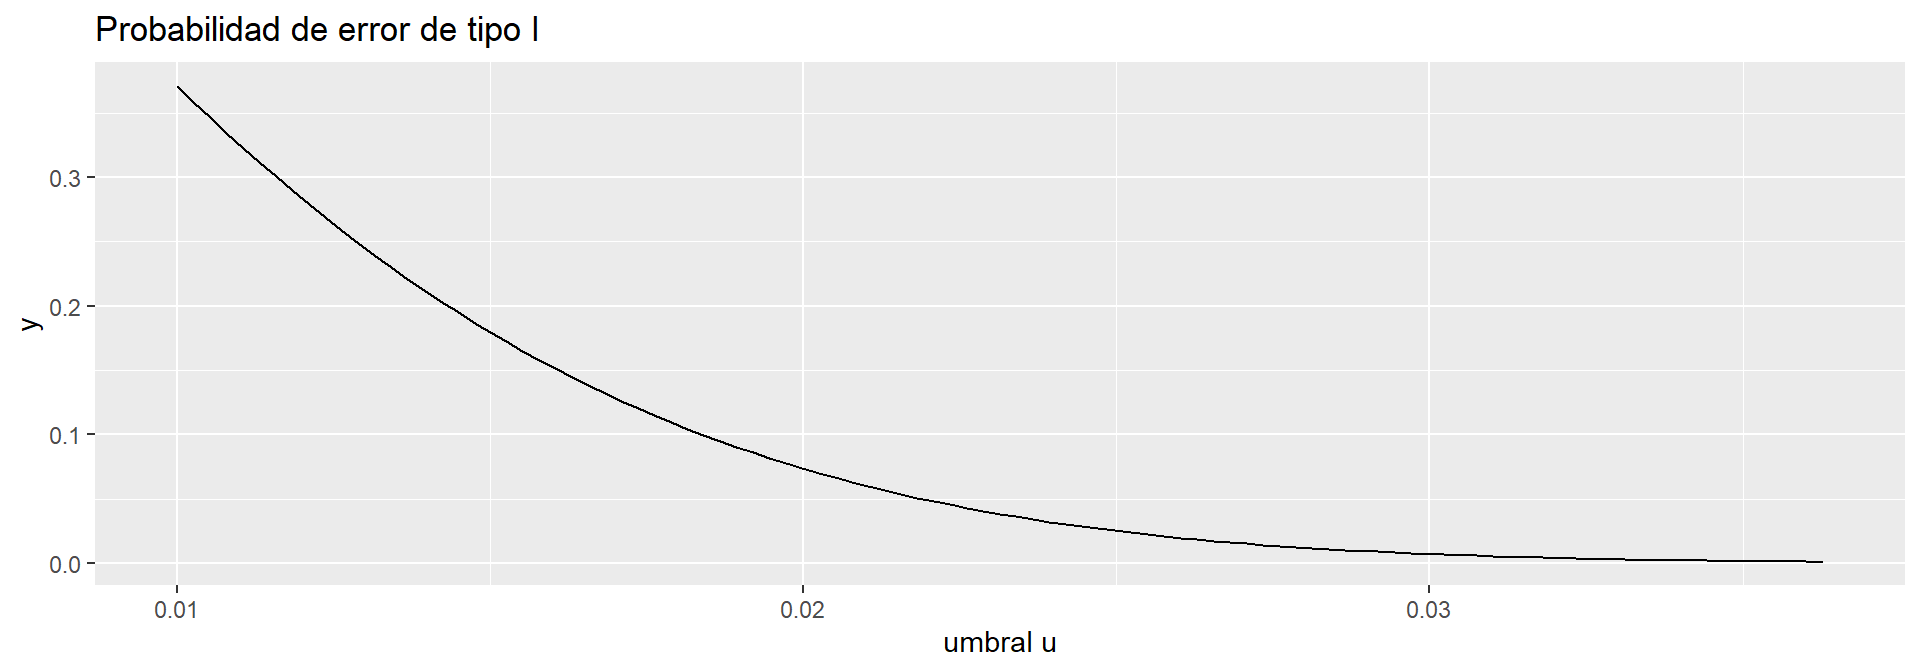
\includegraphics[width=0.7\textwidth]{Tema 4/figures/Figure 1}
\end{center}
Si fijamos $u=0.02$, tenemos una probabilidad de eror de tipo I de 0.05.

¿Qué pasa con la probabilidad de error de tipo II?
 \begin{center}
    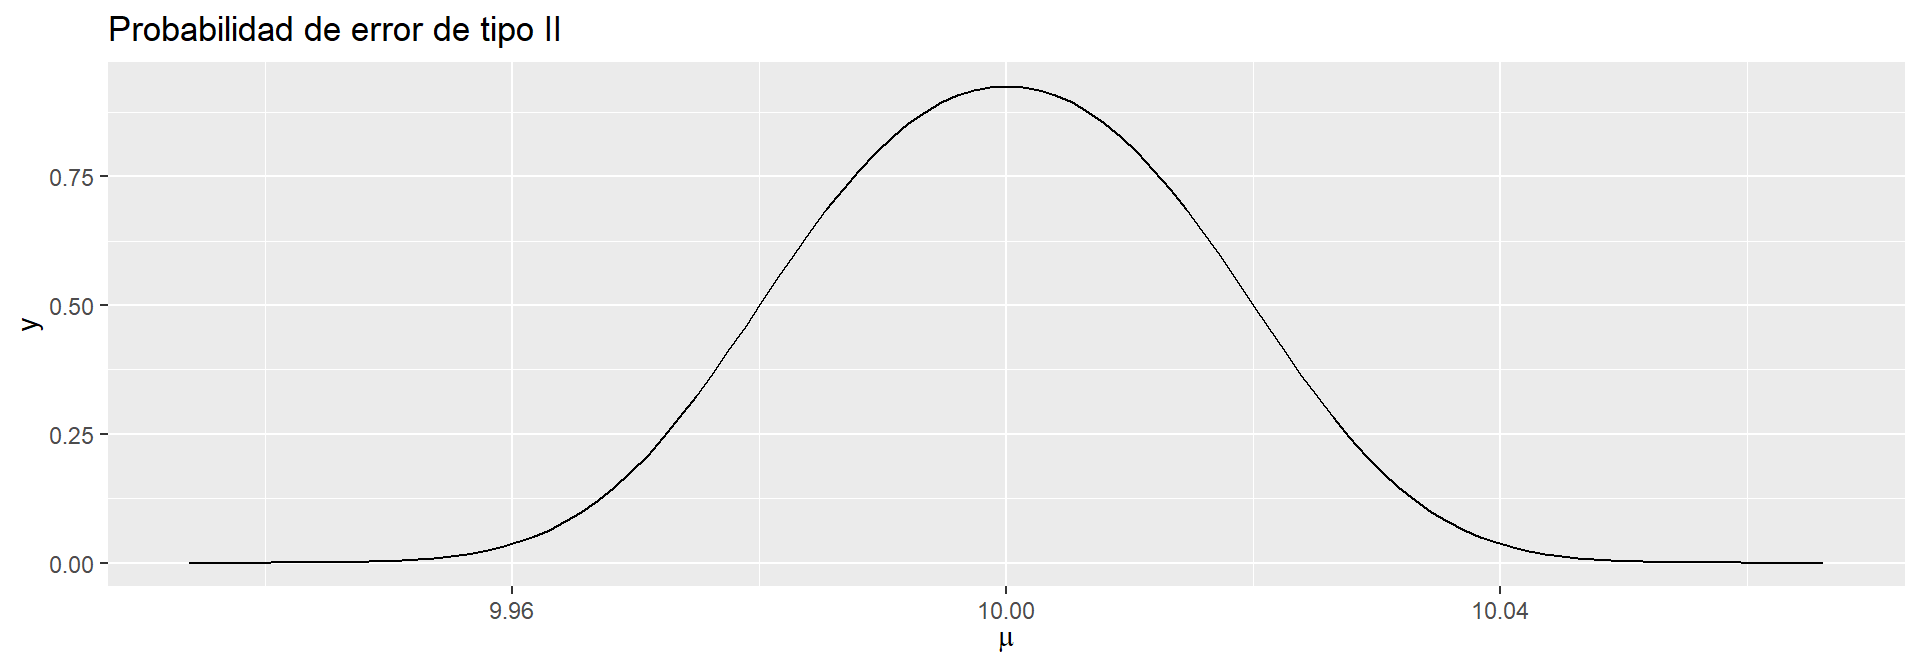
\includegraphics[width=0.7\textwidth]{Tema 4/figures/Figure 2}
\end{center}
Queremos detectar $\mu=10.05$ con una probabilidad suficiente pero a la vez, no queremos rechazar $H_0$ erróneamente con demasiada facilidad.
\begin{center}
    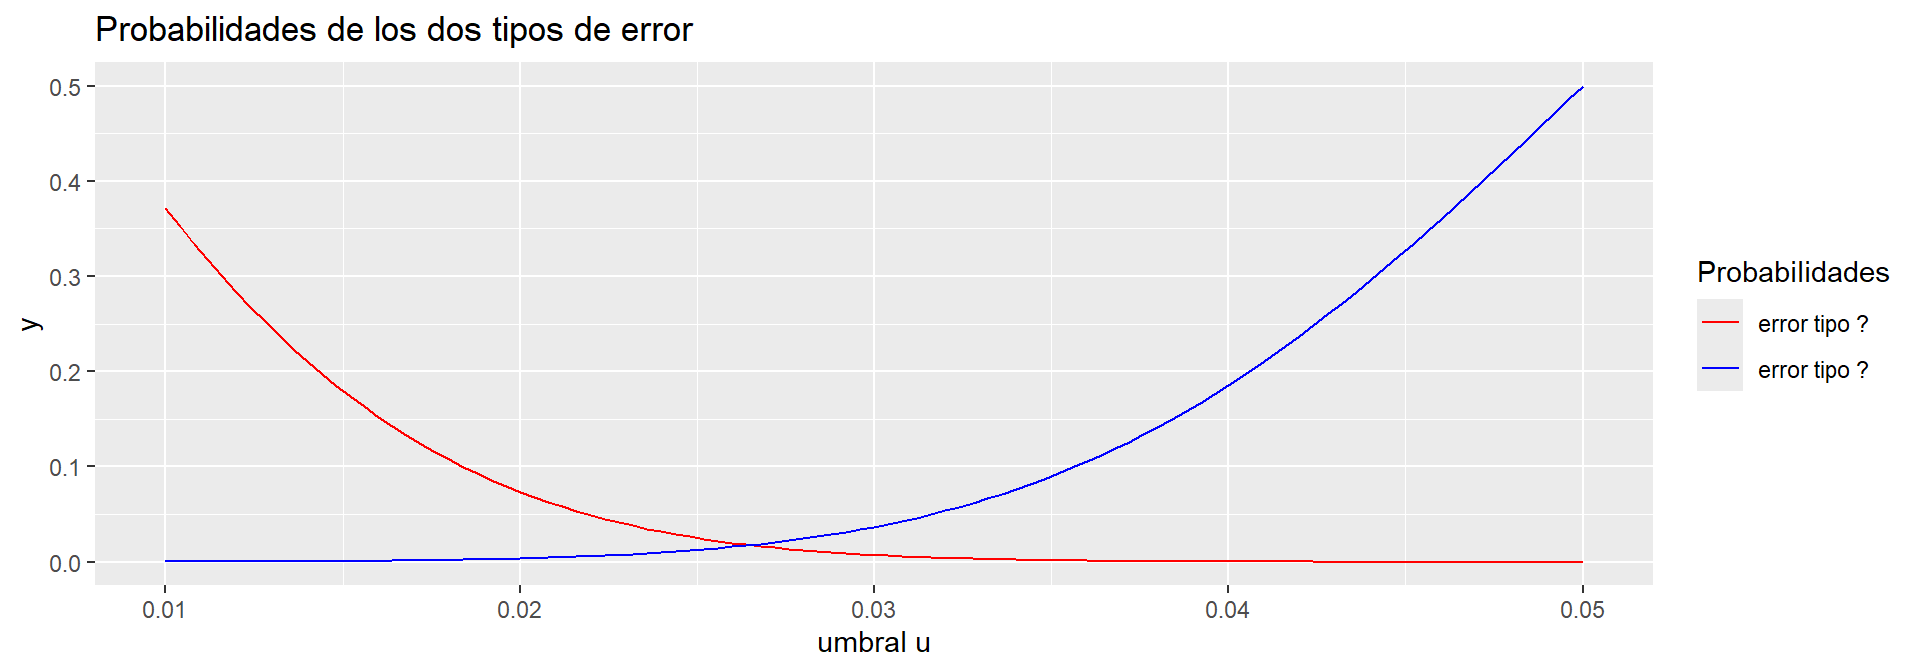
\includegraphics[width=0.7\textwidth]{Tema 4/figures/Figure 3}
\end{center}
\subsection{Métodos útiles para construir tests}
\subsubsection{Un primer procedimiento general}
\begin{tcolorbox}[colback=blue!5!white, colframe=blue!75!black, title=\textbf{Para llevar a cabo un contraste de hipótesis, podemos}]
\begin{itemize}[label=\textbullet]
    \item Formular las hipótesis $H_0$ y $H_1$.
    \item Fijarnos la probabilidad de error de tipo I, $\alpha$.
    \item Para construir nuestra regla $\delta$, escogemos el estadístico de prueba  $T(X_1,\dots,X_n)$ basado generalmente en un estimador del parámetro. Consideramos su distribución muestral suponiendo $H_0$ cierta.
    \item Determinamos la región de rechazo $S_1$, teniendo en cuenta la probabilidad de error I, es decir, \[
    P_{H_0}(T(X_1,\dots,X_n)\in S_1)=\alpha.
    \] 
\item Para nuestra muestra, calculamos $T(x_1,\dots,x_n)$ y decidimos si aceptamos o rechazamos $H_0$, según si su valor está en $S_0$ o en $S_1$.
\end{itemize}
\end{tcolorbox}
\subsection{Constraste de hipótesis para la media $\mu$}
\begin{tcolorbox}[colback=olive!5!white, colframe=olive!75!black, title=\textbf{Primer caso}]
Empezamos por considerar la construcción de un contraste para la media $\mu$ de una población Normal con varianza conocida. 
\end{tcolorbox}
\begin{tcolorbox}[colback=blue!5!white, colframe=blue!75!black, title=\textbf{Contexto}]
\begin{itemize}[label=\textbullet]
    \item Consideramos una v.a. $X$.
    \item Hemos decidido modelar:  $X\sim \mathcal{N}(\mu,\sigma^2)$.

        Tenemos fijado el valor de $\sigma$ (valor poblacional, por ejemplo gracias a datos históricos).
    \item Queremos llevar a cabo un contraste sobre $\mu$.
    \item Para ello, extraeremos una muestra de tamaño $n$ de la distribución de $X$.
\end{itemize}
\end{tcolorbox}
\subsection{Procedimiento, hipótesis bilateral}
\begin{itemize}[label=\textbullet]
    \item Formulamos las hipótesis: \[
    \begin{cases}
        H_0:\mu=\mu_0,\\
        H_1:\mu\neq \mu_0,
    \end{cases}
    \] donde $\mu_0$ representa el valor concreto con el que queremos comparar $\mu$.
\item Fijamos el valor de $\alpha$.
\item El estadístico de prueba es la versión tipificada de $\overline{X}$: \[
Z=\dfrac{\overline{X}-\mu}{\sigma / \sqrt{n} }\sim \mathcal{N}(0,1).
\] 
\item \lb{Si $H_0$ es cierto, $\mu=\mu_0$} \[
Z_0=\dfrac{\overline{X}-\lb{\mu_0} }{\sigma / \sqrt{n} }\sim \mathcal{N}(0,1).
\]  
\item Establecemos la región de rechazo:
\begin{center}
    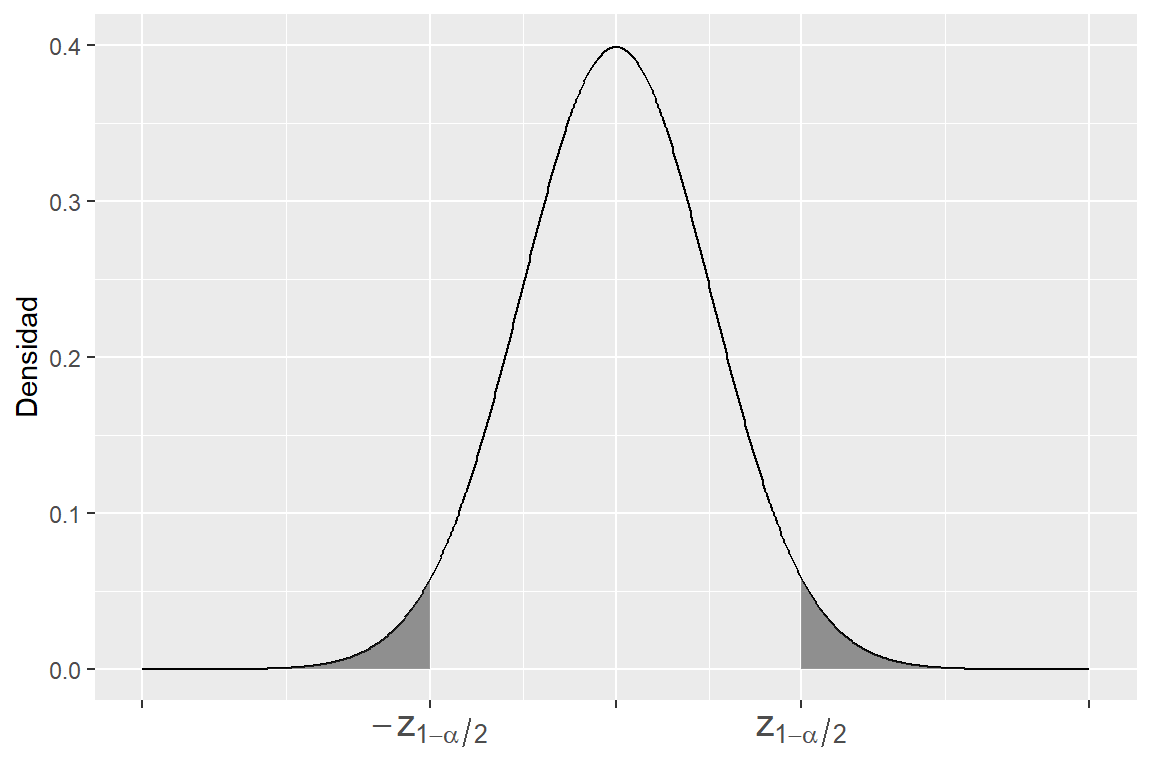
\includegraphics[width=0.7\textwidth]{Tema 4/figures/Figure 4}
\end{center}
La región $S_1$ está formada por los valores menores que $-z_{1-\frac{\alpha}{2} }$ o mayores que $z_{1-\frac{\alpha}{2} }$ .
\item Nos queda calcular, para nuestra muestra, el valor concreto del estadístico de prueba $z_0$:
    \begin{itemize}[label=\textrightarrow]
        \item Si pertenece a $S_1$, rechazaremos $H_0$ y afirmaremos $H_1$.
        \item Si no pertence a $S_1$, admitiremos $H_0$.
    \end{itemize}
\end{itemize}
\subsubsection*{Ejemplo}
\begin{tcolorbox}[colback=blue!5!white, colframe=blue!75!black, title=\textbf{En un proceso de producción}]
\begin{itemize}[label=\textbullet]
    \item La longitud de los artículos producidos se modeliza a través de una distribución Normal con media $\mu$.
    \item Por experiencia acerca del proceso, se cuantifica su desviación típica en $\sigma=1mm$.
    \item En condiciones de funcionamiento correcto, se espera que la longitud media de los artículos sea  $50$ mm.
    \item Para comprobar la calidad se decide tomar una muestra de 10 artículos que resultan tener la longitud media  $\overline{x}$ igual a 51 mm.
    \item Basándonos en esta muestra, ¿qué podemos decir acerca del funcionamiento del proceso?
\end{itemize}
\end{tcolorbox}
\subsection{Procedimiento, hipótesis unilateral}
Todo igual, excepto $S_1$.
\begin{itemize}[label=\textbullet]
    \item Si la hipótesis es $H_1:\mu>\mu_0$, la región de rechazo será
        \begin{center}
            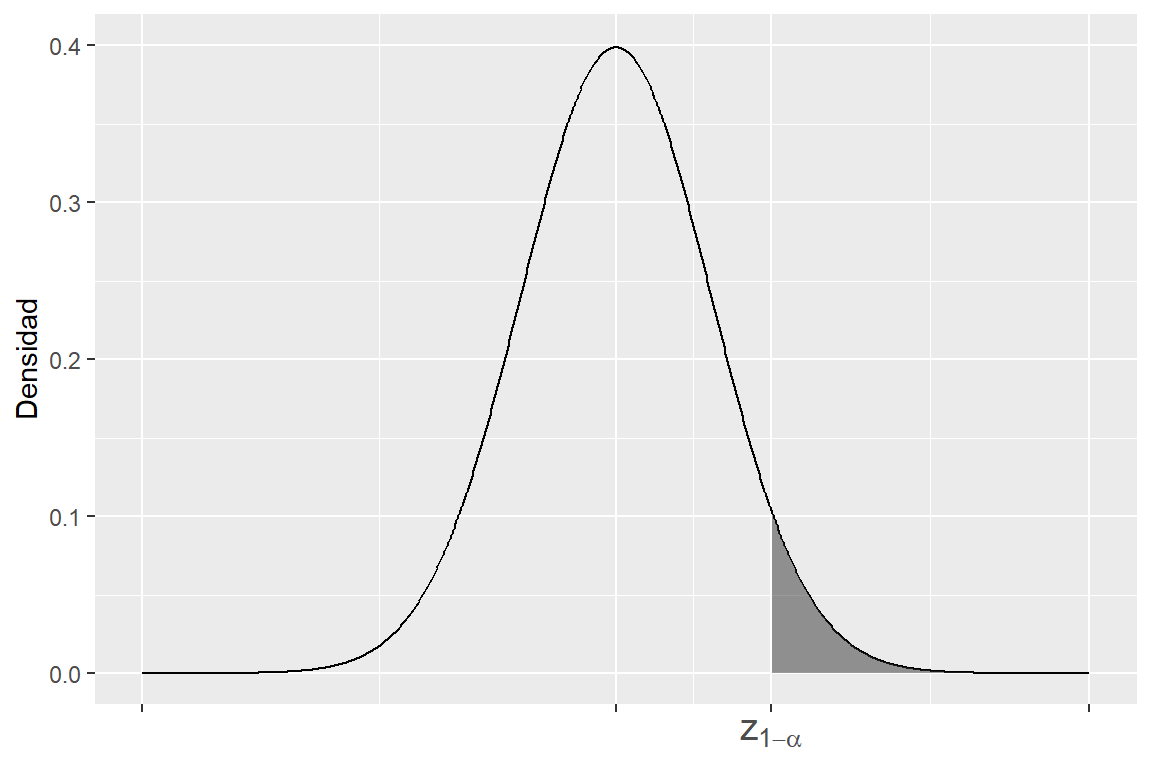
\includegraphics[width=0.7\textwidth]{Tema 4/figures/Figure 5}
        \end{center}
    \item Si la hipótesis es $H_1:\mu<\mu_0$, la región de rechazo será
        \begin{center}
            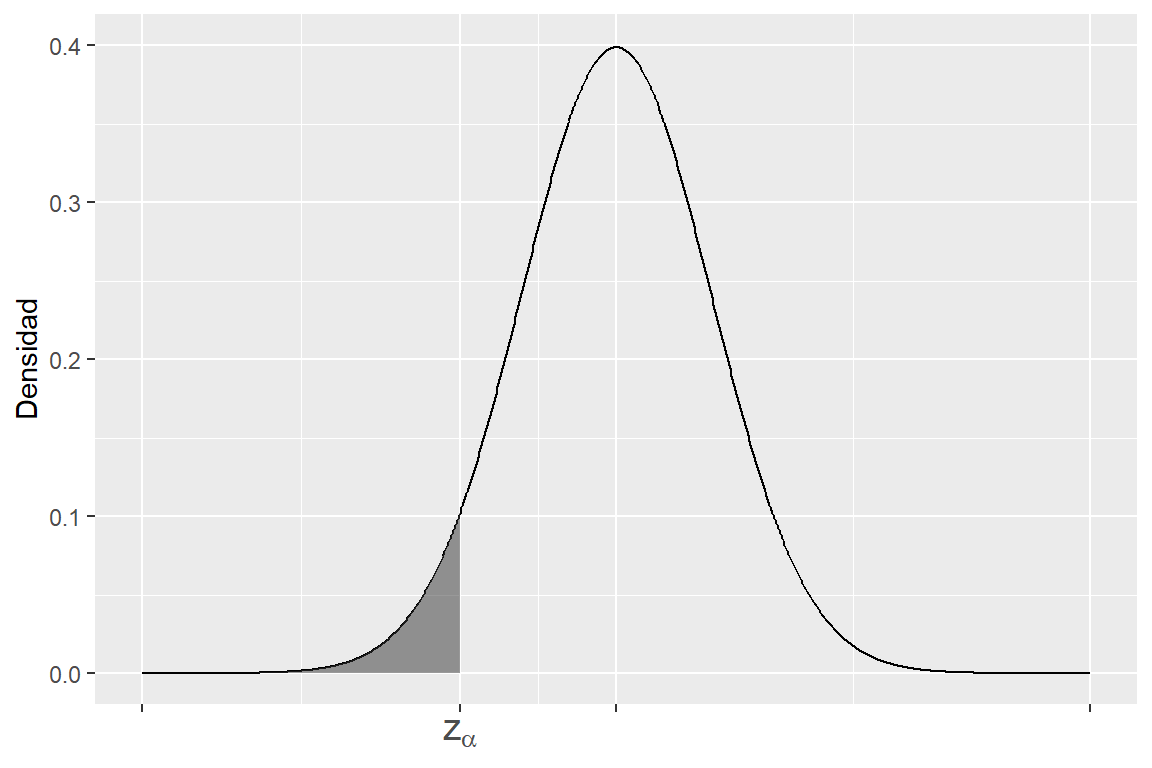
\includegraphics[width=0.7\textwidth]{Tema 4/figures/Figure 6}
        \end{center}
\end{itemize}
\subsection{El p-valor}
\begin{tcolorbox}[colback=blue!5!white, colframe=blue!75!black, title=\textbf{Definición}]
Consideramos un contraste, un test, y hemos observado una muestra concreta $\mathbf{x}$.
\begin{itemize}[label=\textbullet]
    \item El \lb{p-valor} es el nivel de significación más pequeño que nos lleve, para esa muestra $\mathbf{x}$, a rechazar la hipótesis nula.
    \item El p-valor está asociado a la región $S_1$ más pequeñas que nos lleve, para esa muestra, a rechazar $H_0$.
\end{itemize}
\end{tcolorbox}
\begin{tcolorbox}[colback=blue!5!white, colframe=blue!75!black, title=\textbf{Ejemplo}]
Volvamos al ejemplo de la longitud de los artículos producido. Para el contraste \[
    \begin{array}{l}
H_0:\mu=50,\\
        H_1:\mu\neq 50.
    \end{array}
\] Supongamos que hemos encontrado un estadístico de prueba $z_0=1.75$ y rechazamos $H_0$ al 95\% de confianza.

¿Cuál habría sido nuestra decisión al 90\%? ¿Y al 99\% de confianza?
\end{tcolorbox}
\begin{tcolorbox}[colback=olive!5!white, colframe=olive!75!black, title=\textbf{Importante}]
\begin{itemize}[label=\textbullet]
    \item Si rechazamos $H_0$ a un nivel de confianza dado, también la rechazamos a cualquier nivel de confianza menor.
    \item Para saber si la rechazamos a un nivel de confianza mayor, hay que probar.
\end{itemize}
\end{tcolorbox}
\begin{tcolorbox}[colback=blue!5!white, colframe=blue!75!black, title=\textbf{Para calcularlo:}]
\begin{itemize}[label=\textbullet]
    \item Dibujamos la densidad de la distribución muestral del estadístico de prueba.
    \item Colocamos el valor de $z_0$ calculado para mi muestra concreta.
    \item Dibujamos una región de rechazo de manera que $z_0$ coincida con una de las fronteras.
    \item El p-valor $\alpha_0$ es el valor de $\alpha$ correspondiente a esta región de rechazo.
\end{itemize}
\end{tcolorbox}
Para el ejemplo de las longitudes, sabemos $z_0=1.75$, lo colocamos:
\begin{center}
    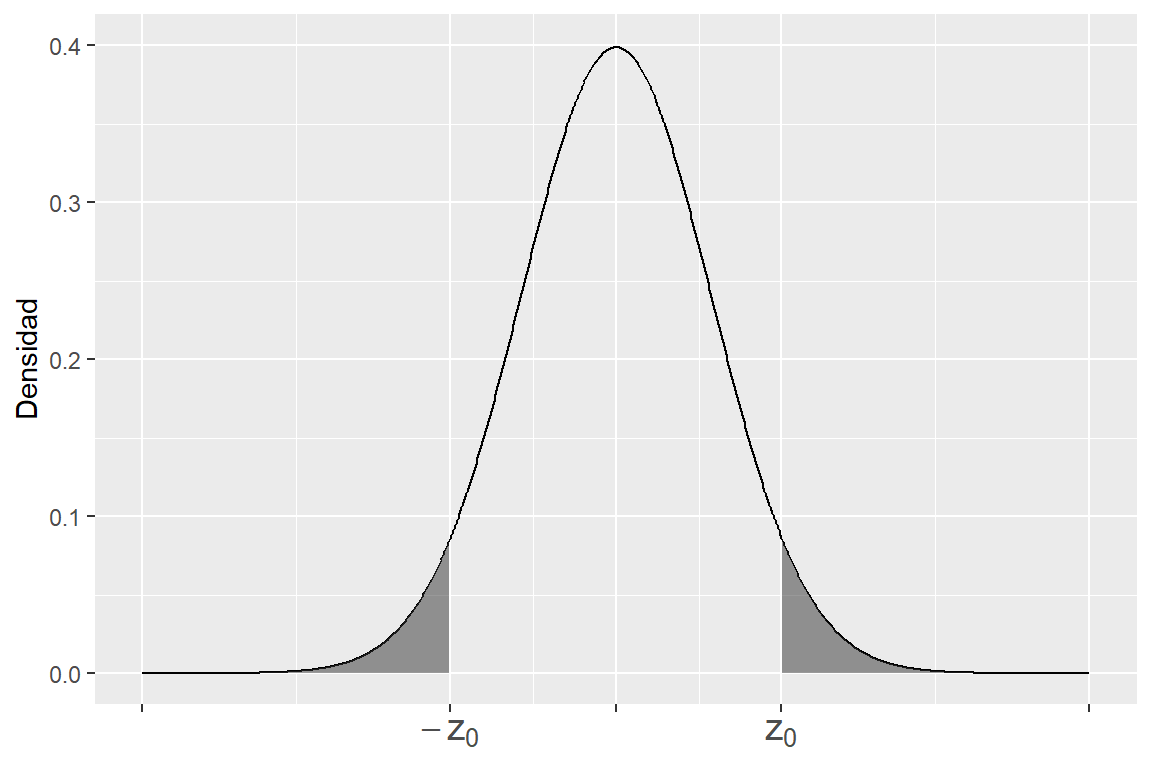
\includegraphics[width=0.7\textwidth]{Tema 4/figures/Figure 7}
\end{center}
Por lo que $\dfrac{\alpha_0}{2}=\mathbb{P}(Z\ge 1.75)$, es decir que $\alpha_0=2(1-\phi(1.75))$, lo que lleva a $\alpha_0\simeq 0.08$.
\begin{tcolorbox}[colback=olive!5!white, colframe=olive!75!black, title=\textbf{Para nuestro ejemplo}]
\begin{itemize}[label=\textbullet]
    \item Encontramos un  p-valor igual a 0.08, por lo que deducimos que la confianza máxima con la que podríamos haber rechazado $H_0$ es del 92\%.
    \item Deducimos que habríamos en particular rechazado $H_0$ al 90\% de confianza, pero, por ejemplo, no al 95\% de confianza.
\end{itemize}
\end{tcolorbox}
\begin{tcolorbox}[colback=olive!5!white, colframe=olive!75!black, title=\textbf{Cuidado con la interpretaión del p-valor}]
El p-valor se puede interpretar como una medida de compatibilidad de los datos con la hipótesis nula.
\begin{itemize}[label=\textbullet]
    \item No debemos usarlo como el único criterio para basar nuestra decisión.
    \item Es bueno hacer gráficas, considerar el contexto, ver si el efecto es relevante y no solamente significativo.
    \item Se debe evitar considerar $p-valor<0.05$ como un valor mágico que es sinónimo de efecto significativo.
\end{itemize}
\end{tcolorbox}
\subsection{Test óptimo}
\begin{tcolorbox}[colback=blue!5!white, colframe=blue!75!black, title=\textbf{Empezamos por considerar los tests con probabilidad de error tipo I menor o igual que $\alpha$:}]
\begin{itemize}[label=\textbullet]
    \item Dado $\alpha$, sea \[
    T_\alpha=\{\delta\in T|P_{i,\delta}(\theta)\le \alpha \text{ para todo }\theta\in \Theta_0\},
    \] llamaremos $\alpha$ el \lb{nivel de significación del test}.
\item Para un test $\delta$, se llama  \lb{tamaño} o \lb{extensión} de $\lambda$ a:  $\sup_{\theta\in \Theta_0}P_{I,\delta}(\theta)$.  
\end{itemize}
\end{tcolorbox}
\begin{tcolorbox}[colback=blue!5!white, colframe=blue!75!black, title=\textbf{Definición}]
Dado $\delta^*\in T_\alpha$ decimos que es \lb{óptimo} si \[
P_{II,\delta^*}(\theta)\le P_{II,\delta}(\theta)\text{ para todo $\delta\in T_\alpha$ y para todo $\theta\in \Theta_1$.}
\]  
\end{tcolorbox}
\subsection{Potencia de un test}
\begin{tcolorbox}[colback=blue!5!white, colframe=blue!75!black, title=\textbf{Definición}]
La \lb{función potencia}  de un test $\delta$ asocia a cada  $\theta$ la probabilidad de rechazar la hipótesis nula:  \[
\theta\mapsto \pi_\delta(\theta)=P_\theta(X \in S_1),\quad \text{con $\theta\in \Theta$}.
\] 
\end{tcolorbox}
\begin{tcolorbox}[colback=olive!5!white, colframe=olive!75!black, title=\textbf{Relación de la potencia con los errores}]
\begin{itemize}[label=\textbullet]
    \item Si $\theta\in \Theta_0$ entonces $\pi_\delta(\theta)=P_{I,\delta}(\theta)$.
    \item Si $\theta\in \Theta_1$ entonces \[
    \pi_\delta(\theta)=P_\theta(X\in S_1)=1-P_\theta(X\in S_0)=1-P_{II,\delta}(\theta).
    \] 
\end{itemize}
\end{tcolorbox}
\subsection{Test óptimo como el de máxima potencia}

Sea $\delta^*\in T_\alpha$, diremos que es el \lb{test uniforme de máxima potencia} para el contraste \[
H_0:\theta\in \Theta
\] frente a \[
H_1:\theta\in \Theta_1
\] si se verifica \[
\pi_{\delta^*})\theta\ge \pi_{\delta}(\theta)\text{ para todo $\delta\in T_\alpha$ y para todo $\theta\in \Theta_1$.}
\] 
\subsection{Procedimientos basados en la verosimilitud}
\begin{tcolorbox}[colback=olive!5!white, colframe=olive!75!black, title=\textbf{Un procedimiento natural}]
Puesto que la verosimilitud expresa la compatibilidad de los datos con el modelo considerado, es natural construir un test basado en la comparación de la verosimilitud para los valores de $\Theta_0$ y para los valores de $\Theta_1$.
\end{tcolorbox}
\begin{tcolorbox}[colback=olive!5!white, colframe=olive!75!black, title=\textbf{Constrastes de hipótesis simples}]
En este tipo de contraste los subconjunto del espacio paramétrico solo tienen un elemento, es decir $\Theta_0=\{\theta_0\} $ y $\Theta_1=\{\theta_1\} $ y por lo tanto los errores de ambos tipos son cantidades fijas. Implícitamente, estamos asumiendo que el parámetro es unidimensional.
\end{tcolorbox}
\subsection{Constrastes de hipótesis simples}
\begin{tcolorbox}[colback=blue!5!white, colframe=blue!75!black, title=\textbf{Lema de Neyman-Pearson}]
Sea $X\sim F(x,\theta),\Theta=\{\theta_0,\theta_1\},\mathbf{X}=(X_1,X_2,\dots,X_n) $, una muestra aleatoria simple de la población $X$,  $\alpha$ fijo con $0<\alpha<1$. Para contrastar la hipótesis nula $H_0:\theta=\theta_0$ frente a la hipótesis alternativa $H_1:\theta=\theta_1$, el test de región de rechazo: \[
S_1=\left\{ \mathbf{x}\in \mathrm{Sop}(\mathbf{X})\bigg|\dfrac{L(\mathbf{x},\theta_1)}{L(\mathbf{x},\theta_0)}\ge k \right\} 
\] con $k>0$, que además tenga tamaño  $\alpha$, es decir $\alpha=P(\mathbf{X}\in S_1|\theta=\theta_0)$, cumple que es el test de máxima potencia en la clase de los tests $T_\alpha$.
\end{tcolorbox}
\begin{itemize}[label=\color{red}\textbullet, leftmargin=*]
    \item \lb{Observaciones}
        \begin{itemize}[label=\textbullet]
            \item Si la distribución es de tipo continuo siempre se cumple que el test alcanza el tamaño obteniéndose el test de extensión de $\alpha$.
            \item Si la distribución es de tipo discreto, en general, el test de máxima potencia será de extensión menor que $\alpha$.
        \end{itemize}
    \item \lb{Demostración} 

        Sea $\delta^*$ el test definido anteriormente.
         \begin{itemize}[label=\textbullet]
            \item La condición \[
            \alpha=P(\mathbf{X}\in S_1|\theta=\theta_0)
            \] nos asegura que $\delta^*\in T_\alpha$. Sea ahora $\delta\in T_\alpha$ cualquiera. Tenemos que probar que: \[
            \pi_{\delta^*}(\theta_1)\ge \pi_{\delta}(\theta_1)
            \] supondremos $X$ variable aleatoria continua (en el caso discreto se razonará de forma análoga).
        \item Sea  $\mathbf{X}\in \mathrm{sop}(X)$ se verifica que: \[
                (\delta^*(\mathbf{X})-\delta(\mathbf{X}))(L(\mathbf{x},\theta_1)-kL(\mathbf{x},\theta_0))\ge 0.
        \] 
    \item Si $\delta(\mathbf{X})^*=1$ entonces: \[
    \dfrac{L(\mathbf{x},\theta_1)}{L(\mathbf{x},\theta_0)}\ge k\longleftrightarrow L(\mathbf{x},\theta_1)-kL(\mathbf{x},\theta_0)\ge 0
    \] y $\delta^*(\mathbf{X})-\delta(\mathbf{X})\ge 0$ ($\delta(\mathbf{X})$ sólo puede ser 0 o 1) y el producto es no negativo.
\item Si $\delta(\mathbf{X})^*=0$ entonces: \[
    \dfrac{L(\mathbf{x},\theta_1)}{L(\mathbf{x},\theta_0)}< k\longleftrightarrow L(\mathbf{x},\theta_1)-kL(\mathbf{x},\theta_0)< 0
\] y $\delta^*(\mathbf{X})-\delta(\mathbf{X})\le 0$ ($\delta(\mathbf{X})$ sólo puede ser 0 o 1) y el producto es no negativo.
\item La integral de la expresión anterior sobre el $\mathrm{sop}(\mathbf{X})$ será no negativa: \[
        \begin{array}{c}
\int_{\mathrm{sop}(\mathbf{X})}(\delta^*(\mathbf{X})-\delta(\mathbf{X}))(L(\mathbf{x},\theta_1)-kL(\mathbf{x},\theta_0))\mathrm{d}\mathbf{x}\ge 0\\ \int_{\mathrm{sop}(\mathbf{X})}\delta^*(\mathbf{X})L(\mathbf{x},\theta_1)\mathrm{d}\mathbf{x}-\int_{\mathrm{sop}(\mathbf{X})}\delta(\mathbf{X})L(\mathbf{x},\theta_1)\mathrm{d}\mathbf{x}-k\int_{\mathrm{sop}(\mathbf{X})}\delta^*(\mathbf{X})L(\mathbf{x},\theta_0)\mathrm{d}\mathbf{x}-\int_{\mathrm{sop}(\mathbf{X})}\delta(\mathbf{X})L(\mathbf{x},\theta_0)\mathrm{d}\mathbf{x}\ge 0
        \end{array}
\] 
notar que ambos contrastes solo toman el valor 1 en sus respectivas regiones de rechazo (y cero en las regiones de aceptación) con lo que al desarrollar los terminos de la integral tenemos: \[
\pi_{\delta^*}-\pi_\delta(\theta_1)-k(\pi_{\delta^*}(\theta_0)-\pi_\delta(\theta_0))\ge 0.
\]
\item Como $\delta\in T_\alpha$ tenemos que $\pi_\delta(\theta_0)\le \alpha$ con lo que: \[
0\le \alpha-\pi_\delta(\theta_0)=\pi_{\delta^*}(\theta_0)-\pi_\delta(\theta_0)
\] y por lo tanto: \[
k(\pi_{\delta^*}(\theta_0)-\pi_\delta(\theta_0))\ge 0
\] con lo que: \[
0\le \pi_{\delta^*}(\theta_1)-\pi_\delta(\theta_1)-k(\pi_{\delta^*}(\delta_0)-\pi_\delta(\theta_0))\le \pi_{\delta^*}(\theta_1)-\pi_\delta(\theta_1)
\] de donde se deduce: \[
\pi_{\delta^*}(\theta_1)\ge \pi_\delta(\theta_1)
\] que era lo que queríamos probar.
        \end{itemize}
\end{itemize}
\subsection{Hipótesis compuestas}
\begin{tcolorbox}[colback=olive!5!white, colframe=olive!75!black, title=\textbf{Planteamiento}]
En las aplicaciones a problemas reales no suelen plantearse, en general, contrastes de hipótesis simple y alternativa simple, pues las hipótesis alternativas no suelen ser tan precisas para que estén definidas por un único valor del parámetro. Consideremos ahora contrastes de hipótesis donde al menos una de ellas es compuesta.
\end{tcolorbox}
\begin{tcolorbox}[colback=blue!5!white, colframe=blue!75!black, title=\textbf{Casos}]
\begin{center}
    \begin{varwidth}{0.5\textwidth}
    \begin{multicols}{2}
   \begin{enumerate}[label=\alph*)]
       \item $\begin{array}{l}
           H_0:\theta=\theta_0\\
           H_1:\theta>\theta_0
       \end{array}$
       \item $\begin{array}{l}
           H_0:\theta=\theta_0\\
           H_1:\theta<\theta_0
       \end{array}$
       \item $\begin{array}{l}
           H_0:\theta\le \theta_0\\
           H_1:\theta>\theta_0
       \end{array}$
       \item $\begin{array}{l}
           H_0:\theta\ge \theta_0\\
           H_1:\theta<\theta_0
       \end{array}$
       \item $\begin{array}{l}
           H_0:\theta=\theta_0\\
           H_1:\theta\neq \theta_0
       \end{array}$
       \item $\begin{array}{l}
               H_0:\theta\in [\theta_1,\theta_2]\\
               H_1:\theta\notin [\theta_1,\theta_2]
       \end{array}$
   \end{enumerate} 
\end{multicols}
\end{varwidth}
\end{center}
En los casos a)-d) anteriores es posible obtener tests uniformes de máxima potencia para casos en los que la variable pertenece a la familia exponencial uniparamétrica.
\end{tcolorbox}
\subsection{Cociente de verosimilitudes monótono}
\begin{tcolorbox}[colback=blue!5!white, colframe=blue!75!black, title=\textbf{Resultado}]
Sea $X\sim F(x,\theta),\theta\in \Theta\subset\R$ y $X_1,\dots,X_n$ una muestra aleatoria simple de $X$. Decimos que  $X$ o  $F$ tienen la propiedad de cociente de verosimilitud monótono en el estadístico  $R=R(X_1,\dots,X_n)$, si para todo $\theta_0,\theta_1\in \Theta$ con $\theta_0<\theta_1$ se verifica que el cociente de verosimilitudes $\dfrac{L(\mathbf{x},\theta_1)}{L(\mathbf{x},\theta)}$, es una función monótona creciente de $R(\mathbf{x})$.
\end{tcolorbox}
\begin{tcolorbox}[colback=red!5!white, colframe=red!75!black, title=\textbf{Nota}]
A los efectos de la definición si $L(\mathbf{x},\theta_0)=0$ y $L(\mathbf{x},\theta_1)>0$, el cociente anterior se considerará igual a infinito.
\end{tcolorbox}
\begin{tcolorbox}[colback=blue!5!white, colframe=blue!75!black, title=\textbf{Familia exponencia uniparamétrica}]
Se dice que la variable $X\sim F(x,\theta)$ pertenece a la familia exponencia uniparamétrica si su función de verosimilitud se puede escribir en la forma: \[
L(\mathbf{x},\theta)=\exp \{A(\theta)T(\mathbf{x})+B(\theta)+h(\mathbf{x})\}
\] para toda muestra $\mathbf{x}$.

Si $A(\theta)$ es monótona creciente (decreciente) en $\theta$, entonces  $X$ tiene cociente de verosimilitud monótono en el estadístico $T(X_1,\dots,X_n)(-T(X_1,\dots,X_n))$.
\end{tcolorbox}

\begin{tcolorbox}[colback=blue!5!white, colframe=blue!75!black, title=\textbf{Cociente de verosimilitudes monótono}]
Sea $X\sim F(x,\theta),\theta\in \Theta\subset \R$ y $X_1,\dots,X_n$ una m.a.s de $X$. Supongamos que  $X$ tiene cociente de verosimilitud monótono en el estadístico $R=R(X_1,\dots,X_n)$ para contrastar $H_0:\theta=\theta_0$ frente a $H_1:\theta>\theta_0$, se sigue que el test \[
\delta_1(\mathbf{x})=\begin{cases}
    0 & \text{si }R(\mathbf{x})<c\\
    1 & \text{si }R(\mathbf{x})\ge c
\end{cases}
\] que cumpla $P_{I,\delta_1}(\theta_0)=\alpha$, es el test uniforme de máxima potencia en la clase de tests $T_\alpha=\{\delta\in T|P_{I,\delta}(\theta_0)\le \alpha\} $, con $0<\alpha<1$.
\end{tcolorbox}
El teorema anterior se extiende al constrante $H_0:\theta\le \theta_0$ frente a $H_1:\theta>\theta_0$.
\begin{tcolorbox}[colback=blue!5!white, colframe=blue!75!black, title=\textbf{Cociente de verosimilitudes monótono}]
Sea $X\sim F(x,\theta),\theta\in \Theta\subset \R$ y $X_1,\dots,X_n$ una m.a.s de $X$. Supongamos que  $X$ tiene cociente de verosimilitud monótono en el estadístico $R=R(X_1,\dots,X_n)$ para contrastar $H_0:\theta=\theta_0$ frente a $H_1:\theta>\theta_0$, se sigue que el test \[
\delta_1(\mathbf{x})=\begin{cases}
    0 & \text{si }R(\mathbf{x})>c\\
    1 & \text{si }R(\mathbf{x})\le c
\end{cases}
\] que cumpla $P_{I,\delta_1}(\theta_0)=\alpha$, es el test uniforme de máxima potencia en la clase de tests $T_\alpha=\{\delta\in T|P_{I,\delta}(\theta_0)\le \alpha\} $, con $0<\alpha<1$.
\end{tcolorbox}
El teorema anterior se extiende al constrante $H_0:\theta\ge \theta_0$ frente a $H_1:\theta<\theta_0$.
\subsection{Constrastes de hipótesis compuesta}
La metodología anterior no se puede aplicar a los casos e) y f) y en los casos de parámetros que no sean unidimensionales. Por tanto, es importante para muchos problemas prácticos, disponer de métodos de construcción de constrastes, basados en principios razonables y que permitan diseñar el test según el problema planteado. El método más importante lo constituye el \textbf{test de la razón de verosimilitudes generalizado}. 
\begin{tcolorbox}[colback=blue!5!white, colframe=blue!75!black, title=\textbf{Razón de verosimilitudes Generalizada (RVG)}]
Se llama razón de verosimilitudes generalizada para constrastar la hipótesis $H_0:\theta\in \Theta$ frente $H_1:\theta\in\Theta_1$ al cociente \[
\lambda(\mathbf{x})=\dfrac{\displaystyle \sup_{\theta\in \Theta_0}L(\mathbf{x};\theta)}{\displaystyle \sup_{\theta\in\Theta_1}L(\mathbf{x};\theta)}.
\] 
\end{tcolorbox}
\subsection{Procedimiento basado en la verosimilitud}
\begin{tcolorbox}[colback=blue!5!white, colframe=blue!75!black, title=\textbf{Test de razón de verosimilitud generalizada}]
Un test de razón de verosimilitud generalizada (RVG) para las hipótesis anteriores es aquel que tiene región crítica de la forma \[
S_1=\left\{ \mathbf{x}\in \mathrm{Sop}(X_1,\dots,X_n)|\lambda(\mathbf{x})=\dfrac{\displaystyle \sup_{\theta\in \Theta_0}L(\mathbf{x};\theta)}{\displaystyle \sup_{\theta\in \Theta}L(\mathbf{x};\theta)}<k \right\} 
\] 
Determinamos la constante $k$, imponiendo que el test tenga extensión $\alpha$, es decir: \[
\sup_{\theta\in\Theta_0}P((X_1,\dots,X_n)\in S_1|\theta)=\alpha.
\] 
\end{tcolorbox}
\subsection{Test RVG para la media de una población normal con varianza conocida}
\begin{tcolorbox}[colback=blue!5!white, colframe=blue!75!black, title=\textbf{Ejercicio}]
\begin{itemize}[label=\textbullet]
    \item $X\sim \mathcal{N}(\mu,\sigma^2)$, suponemos $\sigma$ conocida.
    \item M.a.s  $X_1,\dots,X_n$ de $X$.
    \item Formulamos las hipótesis  \[
            \begin{array}{l}
    H_0:\mu=\mu_0\\
    H_1:\mu\neq \mu_0
            \end{array}
    \] 
\end{itemize}
\begin{enumerate}[label=\arabic*)]
    \item Demostrar que el test que rechaza $H_0$ si $\left| \dfrac{\mathbf{\overline{X}}-\mu_0}{\sigma / \sqrt{n} } \right| >z_{1-\frac{\alpha}{2} }$ es de extensión $\alpha$.
    \item Demostrar que el test anterior es el test de RVG.
\end{enumerate}
\end{tcolorbox}
\textbf{¿Es de extensión $\alpha$?} 
\begin{itemize}[label=\textbullet]
    \item Hemos de comrpboar que: $\sup_{\theta\in \Theta_0}P_{i,\delta}(\theta)=\alpha$.
    \item En este caso $H_0$ es simple, si $\mu=\mu_0$ se cumple que $\dfrac{\mathbf{\overline{X}}-\mu_0}{\sigma / \sqrt{n} }\sim \mathcal{N}(0,1)$. \[
    P\left( \left| \dfrac{\mathbf{\overline{X}}-\mu_0}{\sigma / \sqrt{n} } \right|>z_{1-\frac{\alpha}{2} }|\mu_0  \right) =\alpha.
    \] 
    \begin{center}
        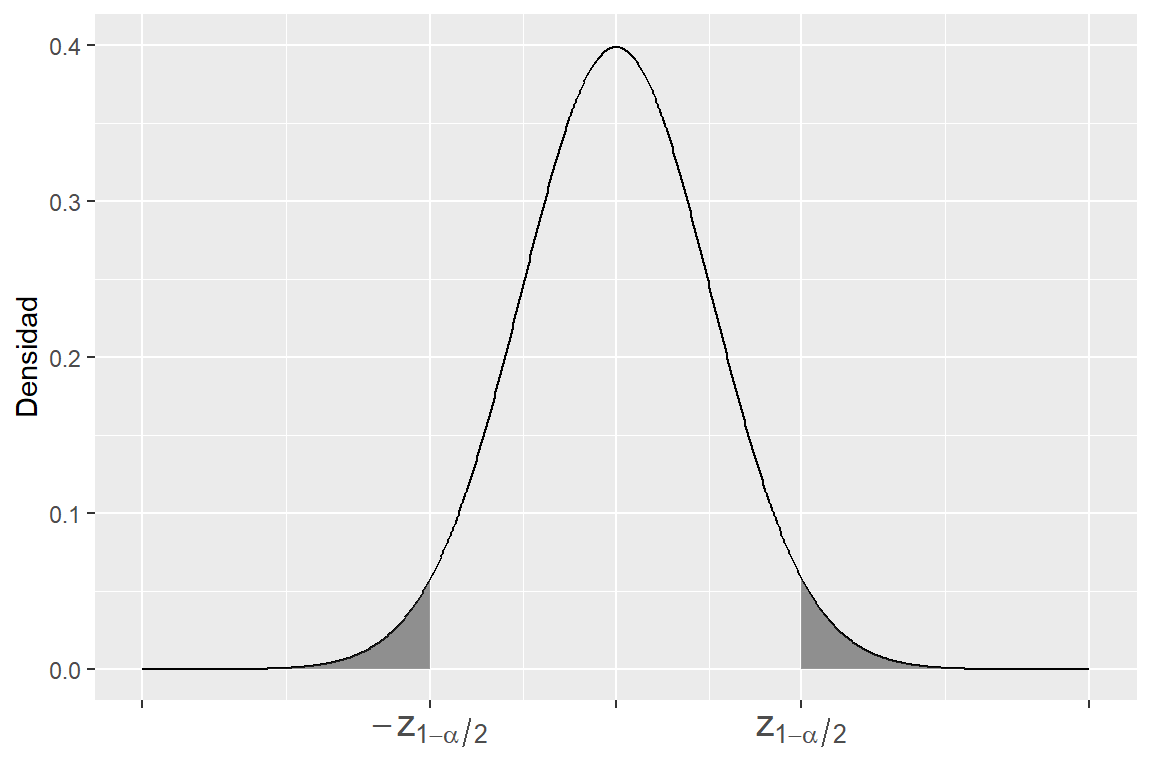
\includegraphics[width=0.7\textwidth]{Tema 4/figures/Figure 4}
    \end{center}
\end{itemize}
\textbf{¿Es el test de RVG?}
\[
\lambda(\mathbf{x})=\dfrac{\displaystyle \sup_{\mu=\mu_0}L(\mathbf{x};\mu)}{\displaystyle \sup_{\mu\in R}L(\mathbf{x};\mu)}.
\] 
\begin{itemize}[label=\textbullet]
    \item Numerador: \[
    L(\mathbf{X};\mu_0)=\dfrac{1}{\sigma^{\frac{n}{2} }(2\pi)^{\frac{n}{2} }}\exp\left( -\dfrac{1}{2\sigma^2}\sum_{i=1}^{n} (x_i-\mu_0)^2 \right) 
    \] 
\item El supremos en el denominador se alcanza en el EMV $\hat{\mu}=\overline{x}_n$.

    \[
        \lambda(\mathbf{x})=\exp\left( -\dfrac{n}{2\sigma^2}\sum_{i=1}^{n} (\overline{x}_n-\mu_0)^2 \right)
    \] 
\end{itemize}
\textbf{¿Es el test de RVG?} 
\begin{itemize}[label=\textbullet]
    \item Determinamos la constante $k$, imponiendo que el test tenga extensión  $\alpha$, es decir, \[
    \begin{array}{c}
        P(\lambda(\mathbf{x})<k|\mu_0)=\alpha\\
        \begin{aligned}
            \alpha&= P\left( 0<\exp\left( -\dfrac{n}{2\sigma^2}\sum_{i=1}^{n} (\overline{x}_n-\mu_0)^2 \right) <k|\mu_0 \right)  \\
            &= P\left( -\infty<-\dfrac{n}{2\sigma^2}\sum_{i=1}^{n} (\overline{x}_n-\mu_0)^2<\log(k)|\mu_0 \right)  \\
            &= P\left( \left( \dfrac{\overline{x}_n-\mu_0}{\sigma / \sqrt{n} } \right) ^2>-2\log(k)|\mu_0 \right)  \\
            &= P\left( \left| \dfrac{\overline{x}_n-\mu_0}{\sigma / \sqrt{n} } \right| >\sqrt{-2\log(k)}|\mu_0  \right)=P\left( \left| \dfrac{\overline{x}_n-\mu_0}{\sigma /\sqrt{n} } \right| >c|\mu_0 \right)   \\
        \end{aligned}
    \end{array}
    \] tomamos $c\impliedby_{1-\frac{\alpha}{2} }$.
\end{itemize}
\subsection{Test de razón de verosimilitudes generalizada}
\begin{tcolorbox}[colback=olive!5!white, colframe=olive!75!black, title=\textbf{Lo más difícil}]
Aunque el test RVG sea un test que suele tener buenas propiedades en cuanto a errores, para muchos modelos, no es sencillo deducir su distribución muestral.
\end{tcolorbox}
\begin{tcolorbox}[colback=blue!5!white, colframe=blue!75!black, title=\textbf{Aproximación asintótica de la distribución muestral para el test RVG}]
Para el contraste \[
H_0:\theta\in \Theta_0
\] frente a la alternativa \[
H_1:\theta\in \Theta_1
\] si $\dim(\Theta)=q$ y  $\dim(\Theta_0)=q'$ se verifica, bajo ciertas condiciones, que el estadístico $-2\log\lambda(\mathbf{X})$ converge en distribución a una ji-cuadrado con $q-q'$ grados de libertad.
\end{tcolorbox}
\subsection{Test de bondad de ajuste}
\begin{tcolorbox}[colback=blue!5!white, colframe=blue!75!black, title=\textbf{Es un contraste no paramétrico}]
\begin{itemize}[label=\textbullet]
    \item Su objetivo es comprobar hasta qué punto los daots observados parecen haber sido generados por una distribución de probabilidad dada.
    \item Se conoce como "contraste chi-cuadrado", porque es la distribución que usamos para construir nuestra regla de decisión.
\end{itemize}
\end{tcolorbox}
\begin{tcolorbox}[colback=blue!5!white, colframe=blue!75!black, title=\textbf{Primer ejemplo, el caso más sencillo:}]
\begin{itemize}[label=\textbullet]
    \item Tenemos $k$ clases posibles asociadas a un experimento aleatorio: $A_1,\dots,A_k$.
    \item Tenemos unos valores esperados para sus probabilidades \[
    p_1=P(A_1),\dots,p_k=P(A_k).
    \] 
\item Observamos $n$ realizaciones del experimento y queremos decidir si lo observado es compatible con los valores esperados.
\end{itemize}
\end{tcolorbox}
\subsection*{Caso sencillo bondad de ajuste}
\begin{tcolorbox}[colback=blue!5!white, colframe=blue!75!black, title=\textbf{El caso más sencillo:}]
\begin{itemize}[label=\textbullet]
    \item Planteamos \[
    \begin{array}{l}
        H_0:P(A_i)=p_i,\,i=1,\dots,k\\
        H_1:\text{Existe $i$ tal que  $P(A_i)\neq p_i$.}
    \end{array}
    \] 
\item Tenemos $k$ clases posibles asociadas a un experimento aleatorio: $A_1,\dots,A_k$.
\item Tenemos unos valores esperados para sus probabilidades \[
p_1=P(A_1),\dots,p_k=P(A_k).
\] 
\item Observamos $n$ realizaciones del experimento y queremos decidir si lo observado es compatible con los valores esperados.
\end{itemize}
\end{tcolorbox}
\subsection*{Caso sencillo bondad de ajuste: grupo sanguíneo}
\begin{tcolorbox}[colback=blue!5!white, colframe=blue!75!black, title=\textbf{Cuatro grupos sanguíneos}]
Experimento: escoger una persona
\begin{itemize}[label=\textbullet]
    \item $A_1=\text{"Su grupo es O"},A_2=\text{"Su grupo es A"},A_3=\text{"Su grupo es B"},A_4=\text{"Su grupo es AB"}.$ 
    \item Los valores esperados para sus probabilidades son $$p_1=43\%,p_2=40\%,p_3=12\%,p_4=5\%.$$ 
    \item En un grupo de 250 personas, observamos $f_1=110\text{ "O", }f_2=100\text{"A"},f_3=30\text{"B"},f_4=10\text{"AB"}$.
    \item En el grupo de 250, esperamos $\hat{f_1}=250\times 43\%\simeq 107.5\text{"O"},\hat{f_2}=2500\times 40\%\simeq 100\text{"A"},\hat{f_3}=250\times 12\%\simeq 30\text{"B"},\hat{f_4}=250\times 5\%\simeq 12.5\text{"AB"}$.
    \item Escribimos los datos en una tabla 
        \begin{center}
            \begin{tabular}{p{2cm}llll}
                \textbf{Clases} & $A_1$ & $A_2$ & $A_3$ & $A_4$\\ \hline
                Frecuencia observada & $f_1=110$ & $f_2=100$ & $f_3=30$ & $f_4=10$\\ \hline
                Frecuencia esperada & $\hat{f_1}=107.5$ & $\hat{f_2}=100$ & $\hat{f_3}=30$ & $\hat{f_4}=12.5$
            \end{tabular}
        \end{center}
\end{itemize}
\end{tcolorbox}
\subsubsection*{Construimos el estadístico para el constraste:}
\begin{tcolorbox}[colback=blue!5!white, colframe=blue!75!black, title=\textbf{El estaístico chi-cuadrado de Pearson}]
Para constrastar \[
\begin{array}{l}
    H_0:P(A_i)=p_i,\:i=1,\dots,k\\
    H_1:\text{Existe $i$ tal que  $P(A_i)\neq p_i$.}
\end{array}
\] 
Karl Pearson propuso el estadístico \[
\chi^2=\sum_{i=1}^{k} \dfrac{\left( f_i-\hat{f_i} \right) ^2}{\hat{f_i}}.
\] 
Si $n$ es suficientemente grande,  \[
\chi^2=\sum_{i=1}^{k} \dfrac{\left( f_i-\hat{f_i} \right) ^2}{\hat{f_i}}\text{ es aprox. $\chi_{k-1}^2$. }
\] 
\end{tcolorbox}
\[
\chi^2=\sum_{i=1}^{k} \dfrac{\left( f_i-\hat{f_i} \right) ^2}{\hat{f_i}}=\dfrac{(100-107.5)^2}{107.5}+\dfrac{0^2}{100}+\dfrac{0^2}{30}+\dfrac{(10-12.5)^2}{12.5}=1.02
\] 
Para calcular el p-valor, lo comparamos con los cuantiles de una $\chi_3^2$, valores extremos positivos nos llevan a rechazar $H_0$.
\begin{tcolorbox}[colback=blue!5!white, colframe=blue!75!black, title=\textbf{p-valor:}]
Encontramos $p-\text{valor}=0.79$, lo que nos lleva a afirmar que los datos apoyan la hipótesis nula, y son compatibls con los valores esperados $p_1=43\%\text{"O"},p_2=40\%\text{"A"},p_3=12\%\text{"B"},p_4=5\%\text{"AB"}$.
\end{tcolorbox}
\begin{tcolorbox}[colback=olive!5!white, colframe=olive!75!black, title=\textbf{Validez de la aproximación de la distribución de estadístico de Pearson por un $\chi_{k-1}^2$.}]
$n$ debe ser "suficientemente" grande.
\begin{itemize}[label=\textbullet]
    \item Se suele considerar que todas las frecuencias esperadas deben ser al menos 5, excepto una, y que esa sea mayor que 0.5.
    \item Si dos de ellas son pequeñas, entonces esas no deben ser menor que 1, y el resto debe ser al menos 5.
    \item Si no se cumple, se agrupan clases.
\end{itemize}
\end{tcolorbox}
\subsubsection*{Segundo caso: debemos estimar parámetros para calcular las frecuencias esperadas.}
\begin{tcolorbox}[colback=blue!5!white, colframe=blue!75!black, title=\textbf{Segundo ejemplo, un caso común:}]
\begin{itemize}[label=\textbullet]
    \item Tenemos $k$ clases posibles asociadas a un experimento aleatorio $A_1,\dots,A_k$.
    \item Los valores esperados para las probabilidades $p_1=P(A_1),\dots,p_k=P(A_k)$ dependen de unos parámetros desconocidos.
    \item Observamos $n$ realizaciones del experimento y queremos decidir si lo observado es compatible con los valores esperados.
    \item Planteamos $H_0:P(A_i)=p_i,\: i=1,\dots,k$ frente a $H_1$: Existe $i$ tal que $P(A_i)\neq p_i$.
\end{itemize}
\end{tcolorbox}
\begin{tcolorbox}[colback=olive!5!white, colframe=olive!75!black, title=\textbf{Procederemos igual que antes, pero:}]
\begin{itemize}[label=\textbullet]
    \item Estimaremos los parámetros desconocidos a partir de las observaciones.
    \item El estadístico de Pearson tendrá como distribución aproximada $\chi_{k-d-1}^2$, donde $d$ es el número de parámetros que debemos estimar para aproximar las frecuencias esperadas.
\end{itemize}
\end{tcolorbox}
\subsubsection*{Ejemplo: daltonismo}
\begin{tcolorbox}[colback=blue!5!white, colframe=blue!75!black, title=\textbf{La incidencia del daltonismo depende del sexo:}]
\begin{itemize}[label=\textbullet]
    \item Los genes responsables del daltonismo se encuentran en el cromosoma $X$.
    \item Los hombres tienen un solo cromosoma  $X\Longrightarrow $ una copia del gen defectuoso en su cromosoma $X$ es suficiente para ser daltónico.
    \item Las mujeres tienen dos cromosomas  $X\Longrightarrow $ dos copias del gen defectuoso son necesarias para ser daltónicas.
\end{itemize}
\end{tcolorbox}
\begin{tcolorbox}[colback=blue!5!white, colframe=blue!75!black, title=\textbf{Si llamamos $q$ a la probabilidad de que el cromosoma  $X$ tenga el gen defectuoso y  $p=1-q$.}]
Tenemos:
\begin{center}
    \begin{tabular}{cll}
      & \textbf{Masculino} & \textbf{Femenino}\\ \hline
        Normales & $\dfrac{p}{2}$ & $\dfrac{p^2}{2}+pq$\\ \hline
        Daltónicos & $\dfrac{q}{2}$ & $\dfrac{q^2}{2}$
 \end{tabular}   
\end{center}
\end{tcolorbox}
\subsection*{Datos observados:}
\begin{tcolorbox}[colback=blue!5!white, colframe=blue!75!black, title=\textbf{Para una muestra de 1000 personas:}]
\begin{center}
    \begin{tabular}{cll}
        & \textbf{Masculino} & \textbf{Feminino} \\ \hline
        Normales & 442 & 514\\
        Daltónicos & 38 & 6\\
    \end{tabular}
\end{center}
\end{tcolorbox}
\newpage
\documentclass{article}
\usepackage{fullpage}
\usepackage[utf8]{inputenc}
\usepackage{pict2e}
\usepackage{amsmath}
\usepackage{enumitem}
\usepackage{eurosym}
\usepackage{mathtools}
\usepackage{amssymb, amsfonts, latexsym, cancel}
\setlength{\parskip}{0.3cm}
\usepackage{graphicx}
\usepackage{fontenc}
\usepackage{slashbox}
\usepackage{setspace}
\usepackage{gensymb}
\usepackage{accents}
\usepackage{adjustbox}
\setstretch{1.35}
\usepackage{bold-extra}
\usepackage[document]{ragged2e}
\usepackage{subcaption}
\usepackage{tcolorbox}
\usepackage{xcolor, colortbl}
\usepackage{wrapfig}
\usepackage{empheq}
\usepackage{array}
\usepackage{parskip}
\usepackage{arydshln}
\graphicspath{ {images/} }
\renewcommand*\contentsname{\color{black}Índice} 
\usepackage{array, multirow, multicol}
\definecolor{lightblue}{HTML}{007AFF}
\usepackage{color}
\usepackage{etoolbox}
\usepackage{listings}
\usepackage{mdframed}
\setlength{\parindent}{0pt}
\usepackage{underscore}
\usepackage{hyperref}
\usepackage{tikz}
\usepackage{tikz-cd}
\usetikzlibrary{shapes, positioning, patterns}
\usepackage{tikz-qtree}
\usepackage{biblatex}
\usepackage{pdfpages}
\usepackage{pgfplots}
\usepackage{pgfkeys}
\addbibresource{biblatex-examples.bib}
\usepackage[a4paper, left=1cm, right=1cm, top=1cm,
bottom=1.5cm]{geometry}
\usepackage{titlesec}
\usepackage{titletoc}
\usepackage{tikz-3dplot}
\usepackage{kbordermatrix}
\usetikzlibrary{decorations.pathreplacing}
\newcommand{\Ej}{\textcolor{lightblue}{\underline{Ejemplo}}}
\setlength{\fboxrule}{1.5pt}

% Configura el formato de las secciones utilizando titlesec
\titleformat{\section}
{\color{red}\normalfont\LARGE\bfseries}
{Tema \thesection:}
{10 pt}
{}

% Ajusta el formato de las entradas de la tabla de contenidos
\addtocontents{toc}{\protect\setcounter{tocdepth}{4}}
\addtocontents{toc}{\color{black}}

\titleformat{\subsection}
{\normalfont\Large\bfseries\color{red}}{\thesubsection)}{1em}{\color{lightblue}}

\titleformat{\subsubsection}
{\normalfont\large\bfseries\color{red}}{\thesubsubsection)}{1em}{\color{lightblue}}

\newcommand{\bboxed}[1]{\fcolorbox{lightblue}{lightblue!10}{$#1$}}
\newcommand{\rboxed}[1]{\fcolorbox{red}{red!10}{$#1$}}

\DeclareMathOperator{\N}{\mathbb{N}}
\DeclareMathOperator{\Z}{\mathbb{Z}}
\DeclareMathOperator{\R}{\mathbb{R}}
\DeclareMathOperator{\Q}{\mathbb{Q}}
\DeclareMathOperator{\K}{\mathbb{K}}
\DeclareMathOperator{\im}{\imath}
\DeclareMathOperator{\jm}{\jmath}
\DeclareMathOperator{\col}{\mathrm{Col}}
\DeclareMathOperator{\fil}{\mathrm{Fil}}
\DeclareMathOperator{\rg}{\mathrm{rg}}
\DeclareMathOperator{\nuc}{\mathrm{nuc}}
\DeclareMathOperator{\dimf}{\mathrm{dimFil}}
\DeclareMathOperator{\dimc}{\mathrm{dimCol}}
\DeclareMathOperator{\dimn}{\mathrm{dimnuc}}
\DeclareMathOperator{\dimr}{\mathrm{dimrg}}
\DeclareMathOperator{\dom}{\mathrm{Dom}}
\DeclareMathOperator{\infi}{\int_{-\infty}^{+\infty}}
\newcommand{\dint}[2]{\int_{#1}^{#2}}

\newcommand{\bu}[1]{\textcolor{lightblue}{\underline{#1}}}
\newcommand{\lb}[1]{\textcolor{lightblue}{#1}}
\newcommand{\db}[1]{\textcolor{blue}{#1}}
\newcommand{\rc}[1]{\textcolor{red}{#1}}
\newcommand{\tr}{^\intercal}

\renewcommand{\CancelColor}{\color{lightblue}}

\newcommand{\dx}{\:\mathrm{d}x}
\newcommand{\dt}{\:\mathrm{d}t}
\newcommand{\dy}{\:\mathrm{d}y}
\newcommand{\dz}{\:\mathrm{d}z}
\newcommand{\dth}{\:\mathrm{d}\theta}
\newcommand{\dr}{\:\mathrm{d}\rho}
\newcommand{\du}{\:\mathrm{d}u}
\newcommand{\dv}{\:\mathrm{d}v}
\newcommand{\tozero}[1]{\cancelto{0}{#1}}
\newcommand{\lbb}[2]{\textcolor{lightblue}{\underbracket[1pt]{\textcolor{black}{#1}}_{#2}}}
\newcommand{\dbb}[2]{\textcolor{blue}{\underbracket[1pt]{\textcolor{black}{#1}}_{#2}}}
\newcommand{\rub}[2]{\textcolor{red}{\underbracket[1pt]{\textcolor{black}{#1}}_{#2}}}

\author{Francisco Javier Mercader Martínez}
\date{}
\renewcommand{\arraystretch}{1}
\setlength{\arraycolsep}{6pt}

\title{Álgebra Lineal\\Ejercicios Tema 4: Subespacios vectoriales, bases y coordenadas}

\begin{document}
\maketitle
\begin{enumerate}[label=\color{red}\textbf{\arabic*)}]
    \item \lb{Determina cuáles de ls siguientes subonjunto de $\R^3$ son subespacios vectoriales:}
        \begin{enumerate}[label=\color{red}\textbf{\alph*)}]
            \item \db{$\{(x,y,z|x=1)\} $} 

                No es un subespacio vectorial porque no contiene al $(0,0,0)$.
            \item \db{$\{(x,y,z)|xyz=0\} $} 

                $W=\{(x,y,z)|xyz=0\} $ 

                Tomamos $(x_1,y_1,z_1),(x_2,y_2,z_2)\in W\longrightarrow \underbrace{(x_1,y_1,z_1)+(x_2,y_2,z_2)}_{(x_1+x_2,y_1+y_2,z_1+z_2)}\in W$ 

                $(x_1+x_2)\cdot (y_1+y_2)\cdot (z_1+z_2)=0$

                Claramente no es un subespacio vectorial porque \textit{"las tres componentes  están multiplicando"} 

                Para verlo más claramente: \[
                \begin{array}{l}
                    v_1=(1,1,0)\in W\text{ ya que }1\cdot 1\cdot 0=0\\
                    v_2=(0,0,1)\in W\text{ ya que }0\cdot 0\cdot 1=0
                \end{array}
                \]
                Sin embargo, $v_1+v_2=(1,1,1)\notin W$ ya que \[
                1\cdot 1\cdot 1=1\neq 0.
                \] 
            \item \db{$\{(x,y,z)|x+y+z=0\} $} 

                $(x_1,y_1,z_1),(x_2,y_2,z_2)\in W\longrightarrow (x_1+x_2,y_1+y_2,z_1+z_2)\in W$

                $(x_1+x_2)+(y_1+y_2)+(z_1+z_2)=\underbrace{(x_1+y_1+z_1)}_{=0}+\underbrace{(x_2+y_2+z_2)}_{=0}=0$

                Sean ahora $(x_1,y_1,z_1)\in W$ y $\alpha\in \R\longrightarrow \alpha(x_1,y_1,z_1)\in W$

                $\begin{array}{l}
                    \alpha(x_1,y_1,z_1)=(\alpha x_1,\alpha y_1,\alpha z_1)\\
                    \alpha x_1+\alpha y_1+\alpha z_1=\alpha\underbrace{(x_1+y_1+z_1)}_{=0}=0
                \end{array}$
        \end{enumerate}
    \item \lb{Comprueba que, en $\R^3$, el subespacio generado por los vectores $(1,2,1)$ y  $(6,1,-16)$ coincide con el subespacio generador por los vectores  $(-3,7,20)$ y  $(4,9,6)$.} 

        Para verificar si el subespacio generador po $\{(1,2,1),(6,1,-16)\} $ coincide con el generado por $\{(-3,7,20),(4,9,6)\} $ en $\R^3$, debemos comprobar si cada conjunto de vectores puede ser expresado como una combinación lineal de los vectores del otro conjunto. Esto implica que ambos subconjuntos generan el mismo campo vectorial.

        Paso a seguir:
        \begin{enumerate}[label=\arabic*)]
            \item \textbf{Matriz ampliada:} Consideramos todos los vectores como filas de una matriz y verificamos si los vectores de un conjunto son combinación lineal de los del otro. Esto se hace calculando las filas escalonadas (rango). \[
            A_1=\begin{bmatrix} 
                1 & 2 & 1\\
                6 & 1 & -16\\
                -3 & 7 & 20\\
                4 & 9 & 6
            \end{bmatrix} 
            \]  
            Reducimos la matriz a su forma escalonada para identificar si el rango es igual a 2 (dimensión de un plano en $\R^3$).
        \item \textbf{Dependencia lineal:} Si se confirma que el rango es 2, probamos si los vectores de un conjunto pertenecen al subespacio generado por los vectores del otro. Para esto, verificamos si existe una relación lineal. 

            $\begin{bmatrix} 
                1 & 2 & 1 \\
                6 & 1 & -16\\
                -3 & 7 & 20\\
                4 & 9 & 6
            \end{bmatrix}\xrightarrow[\begin{subarray}{l}
                F_3\to F_3+3F_1\\
                F_4\to F_4-4F_1
            \end{subarray}]{F_2\to F_2-6F_1}\begin{bmatrix} 
                1 & 2 & 1\\
                0 & -11 & -22\\
                0 & 13 & 23\\
                0 & 1 & 2
            \end{bmatrix}\xrightarrow{F_2\leftrightarrow F_4}\begin{bmatrix} 
                1 & 2 & 1\\
                0 & 1 & 2\\
                0 & 13 & 23\\
                0 & -11 & -22
            \end{bmatrix}\xrightarrow[\begin{subarray}{l}
                F_3\to F_3-13F_2\\
                F_4\to F_4-F_2
            \end{subarray}]{F_1\to F_1-2F_2}\begin{bmatrix} 
                1 & 0 & 3\\
                0 & 1 & 2\\
                0 & 0 & -3\\
                0 & 0 & 0
            \end{bmatrix}\xrightarrow{F_3\to -\frac{1}{3} F_3}\begin{bmatrix} 
                1 & 0 & -3\\
                0 & 1 & 2\\
                0 & 0 & 1\\
                0 & 0 & 0
            \end{bmatrix}\xrightarrow[F_2\to F_2-2F_3]{F_1\to F_1+3F_3}\begin{bmatrix} 
                1 & 0 & 0\\
                0 & 1 & 0\\
                0 & 0 & 1\\
                0 & 0 & 0
            \end{bmatrix}$

            La matriz tiene rango 3, lo cual indica que los cuatro vectores son linealmente independientes. Por lo tanto, los subespacios generados por los conjuntos $\{(1,2,1),(6,1,-16)\} $ y $\{(-3,7,20),(4,9,6)\} $ \textbf{no coinciden}, ya que el espacio generado por los cuatro vectores abarca todo $\R^3$. 
            
        \end{enumerate}

\item \lb{Usando determinantes, halla una base del subespacio $W$ del ejercicio anterior que esté contenida en el conjunto generador dado.}

    \item \lb{Sean $v_1,v_2,v_3\in \mathbb{K}^n$ con $n\ge 3$. Pon un ejemplo de una matriz $A$ tal que los sistemas de ecuaciones $Ax=v_1$ y $Ax=v_2$ tengan solución pero el sistema $Ax=v_3$ no lo tenga.}

        
        Para encontrar un ejemplo de una matriz $A$ en $\mathbb{K}^{n\times n}$ (donde $\mathbb{K}$ es un cuerpo, como $\R$ o $\mathbb{C}$), junto con vectore $v_1,v_2,v_3\in \mathbb{K}^n$, tal que:
        \begin{enumerate}[label=\arabic*)]
            \item $Ax=v_1$ y $Ax=v_2$ tienen solución.
            \item $Ax=v_3$ no tiene solución.
        \end{enumerate}
        Seguimos estos pasos:

        \textbf{Construcción del ejemplo:}
        \begin{enumerate}[label=\arabic*)]
            \item Para que $Ax=v_1$ y $Ax=v_2$ tengan solución, los vectores $v_1$ y $v_2$ deber pertenecer al espacio columnas de $A$, es decir,  $\mathrm{Im}(A)$.
            \item Para que $Ax=v_3$ no tenga solución, $v_3$ debe estar fuera del espacio columna de $A$.
        \end{enumerate}

        Supongamos que $A\in \R^{3\times 3}$, con rango 2 (por simplicidad). Esto implica que $\mathrm{Im}(A)$ es un subespacio de dimensión $2$ en  $\R^3$.

        Sea: \[
        A=\begin{bmatrix} 
            1 & 0 & 0\\
            0 & 1 & 0\\
            0 & 0 & 0
        \end{bmatrix} .
        \] 
        \begin{enumerate}[label=\arabic*)]
            \item \textbf{Espacio columna de $A$:} El espacio columna de $A$ está generado por $\{(1,0,0),(0,1,0)\} $, que es un subespacio de $\R^3$ de dimensión 2.

            \item \textbf{Elegir $v_1$ y $v_2$ dentro de $\mathrm{Im}(A)$:} Escogemos $v_1=(1,1,0)$ y $v_2=(2,-1,0)$, ambos en $\mathrm{Im}(A)$.
            \item \textbf{Elegir $v_3$ fuera de $\mathrm{Im}(A)$:} Escogemos $v_3=(0,0,1)$, que no pertenece a $\mathrm{Im}(A)$, ya que su componente en la tercera coordenada es no nula y la tercera fila de $A$ es cero.
        \end{enumerate}
        \textbf{Verificación}
        \begin{enumerate}[label=\arabic*)]
            \item \textbf{Sistemas $Ax=v_1$ y $Ax=v_2$:} El sistema $Ax=v_1$ tiene solución porque $v_1\in \mathrm{Im}(A)$. Por ejemplo, una solución es: \[
            v_1=\begin{bmatrix} 
            1\\
            1\\
            0
            \end{bmatrix} .
            \]
            Similarmente, $Ax=v_2$ tiene solución, como: \[
            v_2=\begin{bmatrix} 
            2\\
            -1\\
            0
            \end{bmatrix} .
            \] 
        \item \textbf{Sistema $Ax=v_3$:} No tiene solución porque $v_3=(0,0,1)$ no pertence al espacio columna de $A$, que está contenido en el plano $\{(x,y,0)|x,y\in \R\} $.
        \end{enumerate}
    \item \lb{Completa la frase "el vector $b$ pertenece a $\mathrm{Col}(A)$ cuando \dots\dots tiene solución".}

        El vector $b$ pertenece a $\mathrm{Col}(A)$ cuando \textbf{el sistema de ecuaciones lineales $Ax=b$} tiene solución.
    \item \lb{Cierto o falso: "si el vector cero pertenece a $\mathrm{Fil}(A)$, entonces las filas de $A$ son linealmente dependientes".}

        \textbf{Cierto.}

        Si el vector cero pertenece a $\mathrm{Fil}(A)$ (el espacio fila de $A$), significa que al menos una de las filas de $A$ es el vector cero. Esto implica automáticamente que las filas de $A$ son linealmente dependientes, porque cualquier conjunto de vectores que incluya el vector cero no puede ser linealmente independiente.
    \item \lb{Halla una base del subespacio vectorial $W$ de $\R^5$ generado por los vectores \[
                (-1,0,0,1,-2)\quad(2,1,0,-1,2)\quad(1,3,1,0,-1)\quad(0,2,1,0,-1)\quad(3,1,0,-2,4).
    \] } 

    Para hallar una base del subespacio $W\subset \R^5$ generado por los vectores dados, necesitamos determinar un conjunto de vectores linealmente independientes que generen $W$. Esto lo logramos aplicando reducción por filas a la matriz formada por estos vectores.
    \[
    A=\begin{bmatrix} 
        -1 & 0 & 0 & 1 & -2 \\
        2 & 1 & 0 & -1 & 2\\
        1 & 3 & 1 & 0 & -1\\
        0 & 2 & 1 & 0 & -1\\
        3 & 1 & 0 & -2 & 4
    \end{bmatrix} 
    \] 
$\begin{aligned}
\begin{bmatrix} 
        -1 & 0 & 0 & 1 & -2 \\
        2 & 1 & 0 & -1 & 2\\
        1 & 3 & 1 & 0 & -1\\
        0 & 2 & 1 & 0 & -1\\
        3 & 1 & 0 & -2 & 4
    \end{bmatrix}&\xrightarrow{F_1\to -F_1}\begin{bmatrix} 
        1 & 0 & 0 & -1 & 2 \\
        2 & 1 & 0 & -1 & 2\\
        1 & 3 & 1 & 0 & -1\\
        0 & 2 & 1 & 0 & -1\\
        3 & 1 & 0 & -2 & 4
        \end{bmatrix}\xrightarrow[\begin{subarray}{l}
            F_3\to F_3-F_1\\
            F_5\to F_5-3F_1
    \end{subarray}]{F_2\to F_2-2F_1}\begin{bmatrix} 
        1 & 0 & 0 & -1 & 2\\
        0 & 1 & 0 & 1 & -2\\
        0 & 3 & 1 & 1 & -3\\
        0 & 2 & 1 & 0 & -1\\
        0 & 1 & 0 & 1 & -2
    \end{bmatrix}\\ 
& \xrightarrow[\begin{subarray}{l}
        F_4\to F_4-2F_2\\
        F_5\to F_5-F_2
    \end{subarray}]{F_3\to F_3-3F_2} \begin{bmatrix} 
        1 & 0 & 0 & -1 & 2\\
        0 & 1 & 0 & 1 & -2\\
        0 & 0 & 1 & -2 & 3\\
        0 & 0 & 1 & -2 & 3\\
        0 & 0 & 0 & 0 & 0\\
    \end{bmatrix}\xrightarrow{F_4\to F_4-F_3}\begin{bmatrix} 
        1 & 0 & 0 & -1 & 2\\
        0 & 1 & 0 & 1 & -2\\
        0 & 0 & 1 & -2 & 3\\
        0 & 0 & 0 & 0 & 0\\
        0 & 0 & 0 & 0 & 0
    \end{bmatrix} \end{aligned} $

    Tomamos las filas originales correspondientes a las posiciones de los pivotes $(v_1,v_2,v_3)$: \[
    \text{Base de }W=\{(-1,0,0,1,-2),(2,1,0,-1,2),(1,3,1,0,-1)\} .
    \] 
    \item \lb{Amplía el conjunto $\{(1,-1,1)\} $ a una base ortonormal de $\R^3$.}

Para ampliar el conjunto $\{(1,-1,1)\} $ a una base ortonormal de $\R^3$, seguiremos los pasos utilizando el proceso de \textbf{Gram-Schmidt} y la normalización. El objetivo es encontrar dos vectores ortogonales adicionales, completar la base y normalizar todos los vectores.

       \begin{enumerate}[label=Paso \arabic*:]
           \item Normalizamos el primer vector

               El vector dado es $v_1=(1,-1,1)$. Calculamos su norma: \[
               \|v_1\|=\sqrt{1^2+(-1)^2+1^2}= \sqrt{3}. 
               \] 
               Normalizamos $v_1$: \[
               e_1=\dfrac{v_1}{\|v_1\|}=\left( \dfrac{1}{\sqrt{3} },-\dfrac{1}{\sqrt{3} },\dfrac{1}{\sqrt{3} } \right) .
               \] 
           \item Escogemos un vector independiente para construir el siguiente

               Escogemos $v_2=(1,1,0)$, que no es paralelo a $v_1$. Proyectamos $v_2$ sobre $e_1$ y restamos para garantizar ortogonalidad: \[
               \text{Proyección de $v_2$ sobre $e_1=\left<v_2,e_1 \right>e_1$.}
               \] 
               Calculamos: \[
               \left<v_2,e_1 \right> = 1\cdot \dfrac{1}{\sqrt{3} }+1\cdot \left( -\dfrac{1}{\sqrt{3} } \right) +0\cdot \dfrac{1}{\sqrt{3} }=0.
               \] 
               Dado que la proyección es cero, $v_2$ ya es ortogonal a $v_1$. Continuamos con $v_2$ sin cambios: \[
               u_2=v_2=(1,1,0).
               \] 
               Normalizamos $u_2$: \[
               \|u_2\|=\sqrt{1^2+1^2+0^2}=\sqrt{2},\quad e_2=\dfrac{u_2}{\|u_2\|}=\left( \dfrac{1}{\sqrt{2} },\dfrac{1}{\sqrt{2} },0 \right).
               \] 
           \item Encontramos el tercer vector ortogonal

               Escogemos $v_3=(0,0,1)$, que es independiente de $v_1$ y $v_2$. Proyectamos $v_3$ sobre $e_1$ y $e_2$ para garantizar ortogonalidad: \[
               \text{Proyección de $v_3$ sobre $e_1=\left<v_3,e_1 \right>e_1$,}\quad \text{Proyección de $v_3$ sobre $e_2=\left<v_3,e_2 \right>e_2$.}
               \] 
               Calculamos: \[
               \begin{array}{c}
                   \left<v_3,e_1 \right> = 0\cdot \dfrac{1}{\sqrt{3} }+0\cdot \left( -\dfrac{1}{\sqrt{3} } \right) +1\cdot \dfrac{1}{\sqrt{3} }=\dfrac{1}{3},\\
                   \left<v_3,e_2 \right> = 0\cdot \dfrac{1}{\sqrt{2} }+0\cdot \dfrac{1}{\sqrt{2} }+1\cdot 0=0.
               \end{array}
               \] 
               Entonces: \[
               \text{Proyección total: }\dfrac{1}{\sqrt{3} }e_1=\dfrac{1}{\sqrt{3} }\left( \dfrac{1}{\sqrt{3} },-\dfrac{1}{\sqrt{3} },\dfrac{1}{\sqrt{3} } \right) =\left( \dfrac{1}{3},-\dfrac{1}{3},\dfrac{1}{3} \right) .
               \] 
               Restamos esta proyección de $v_3$: \[
               u_3=v_3-\text{Proyección total}=(0,0,1)-\left( \dfrac{1}{3},-\dfrac{1}{3},\dfrac{1}{3} \right) =\left( -\dfrac{1}{3},\dfrac{1}{3},\dfrac{2}{3} \right) .
               \] 
               Normalizamos $u_3$: \[
               \begin{array}{c}
                   \|u_3\|=\sqrt{\left( -\dfrac{1}{3} \right) ^2+\left( \dfrac{1}{3} \right) ^2+\left( \dfrac{2}{3} \right) ^2}=\sqrt{\dfrac{1}{9}+\dfrac{1}{9}+\dfrac{4}{9}} =\sqrt{\dfrac{6}{9}} =\sqrt{\dfrac{2}{3}} . \\
                   e_3=\dfrac{u_3}{\|u_3\|}=\left( -\dfrac{1}{\sqrt{6} },\dfrac{1}{\sqrt{6} },\dfrac{2}{\sqrt{6} } \right) 
               \end{array}
               \] 
       \end{enumerate}
       \textbf{Base ortonormal completa:} \[
       \mathcal{B}=\left\{ \left( \dfrac{1}{\sqrt{3} },-\dfrac{1}{\sqrt{3} },\dfrac{1}{\sqrt{3} } \right) ,\left( \dfrac{1}{\sqrt{2} },\dfrac{1}{\sqrt{2} },0 \right) ,\left( -\dfrac{1}{\sqrt{6} },\dfrac{1}{\sqrt{6} },\dfrac{2}{\sqrt{6} } \right)  \right\} .
       \]  
    \item \lb{En $\R^5$, si las ecuaciones del subespacio $U$ son $\left\{ \begin{array}{l}
        x+y+z+t+u=0\\
        x-y+z-t+u=0
    \end{array} \right\} $, encuentra las de $U^{\perp}$.}

        \textbf{Propiedades de $U$ y $U^\perp$:}
        \begin{enumerate}[label=\arabic*)]
            \item Un vector $v=(x,y,z,t,u)\in U^\perp$ pertenece al subespacio ortogonal si y solo si satisface: \[
            \left<v,w \right> = 0\quad \forall w\in U.
            \] 
            Es decir, $v$ es ortogonal a todos los vectores de $U$.
        \item Si $U$ está definido por $m$ ecuaciones, el rago del sistema de ecuaciones es $m$, y la dimensión de $U$ es $n-m$, donde  $n=5$ en este caso. El subespacio ortogonal  $U^\perp$ tendrá dimensión  $m$.
        \end{enumerate}
        \begin{enumerate}[label=Paso \arabic*:]
            \item Escribir las ecuaciones de $U$ en forma matricial

                Las ecuaciones de $U$ puede escribirsr como un sistema lineal: \[
                \begin{bmatrix} 
                    1 & 1 & 1 & 1 & 1\\ 
                    1 & -1 & 1 & -1 & 1\\ 
                \end{bmatrix} \begin{bmatrix} 
                x\\
                y\\
                z\\
                t\\
                u
                \end{bmatrix} =\begin{bmatrix} 
                0\\ 0 
                \end{bmatrix} .
                \] 
                La matriz de coeficientes es: \[
                A=\begin{bmatrix} 
                    1 & 1 & 1 & 1 & 1\\ 
                    1 & -1 & 1 & -1 & 1\\ 
                \end{bmatrix} .
                \] 
            \item Calcular el espacio nulo de $A$

                El subespacio  $U^\perp$ está generado por los vectores que forma una base del espacio fila de  $A$. Esto corresponde a calcular el espacio nulo de $A^\intercal$, donde: \[
                A^\intercal=\begin{bmatrix} 
                    1 & 1 \\
                    1 & -1\\
                    1 & 1\\
                    1 & -1\\
                    1 & 1
                \end{bmatrix} .
                \] 
                Resolvemos $A^\intercal v=0$, es decir: \[
                \begin{aligned}
                    v_1+v_2+v_3+v_4+v_5&= 0 \\
                    v_1-v_2+v_3-v_4+v_5&= 0 \\
                \end{aligned}
                \] 
            \item Simplificar el sistema

                Sumamos ambas ecuaciones: \[
                2v_1+2v_3+2v_5=0\longrightarrow v_1+v_3+v_5=0.
                \] 
                Restamos ambas ecuaciones: \[
                2v_2+2v_4=0\longrightarrow v_2+v_4=0.
                \] 
                El sistema simplificado es: \[
                \begin{aligned}
                    v_1+v_3+v_5&= 0 \\
                    v_2+v_4&= 0 \\
                \end{aligned}
                \] 
            \item Conclusión

                Las ecuaciones del subespacio $U^\perp$ son: \[
                \begin{aligned}
                    x+z+u&= 0 \\
                    y+t&= 0 \\
                \end{aligned}
                \] 
        \end{enumerate}
    \item \lb{Halla una base de siguientes subespacios vectoriales de $\R^4$:}
        \begin{enumerate}[label=\color{red}\textbf{\alph*)}]
            \item \db{$\{(x,y,z,t)|x=y=z=t\} $} 

                El subespacio está formado por los vectores de la forma $(x,x,x,x)$, donde  $x\in \R$. Esto indica que cualquier vector en este subespacio es un múltiplo del vector $(1,1,1,1)$.

                El subespacio es unidimensional, ya que cualquier vector puede escribirse como: \[
                    (x,x,x,x)=x\cdot (1,1,1,1).
                \] 
                Por lo tanto, una base del subespacio es: \[
                \mathcal{B}=\{(1,1,1,1)\} .
                \] 
            \item \db{$\{(x,y,z,t)|x+y+z+t=0\} $} 
                
                El subespacio $U$ está definido por una ecuación lineal homogénea en $\R^4$, por lo que es un subespacio de dimensión $4-1=3$. Queremos encontrar una base para este subespacio.
                 \begin{enumerate}[label=Paso \arabic*:]
                    \item Representación de los vectores en $U$ 

                        La ecuación $x+y+z+t=0$ implica que:  \[
                        x=-y-z-t.
                        \] 
                        Podemos parametrizar los vectores en $U$ en términos de $y,z,$ y  $t$:  \[
                            (x,y,z,t)=(-y-z-t,y,z,t).
                        \] 
                        Reescribiendo: \[
                            (x,y,z,t)=y(-1,1,0,0)+z(-1,0,1,0)+t(-1,0,0,1).
                        \] 
                    \item Vectores generados

                        Los vectores generadores de $U$ son: \[
                        v_1=(-1,1,0,0),\quad v_2=(-1,0,1,0),\quad v_3=(-1,0,0,1).
                        \] 
                    \item Conclusión

                        Una base del subespacio $U$ es: \[
                        \mathcal{B}=\{(-1,1,0,0),(-1,0,1,0),(-1,0,0,1)\} .
                        \] 
                \end{enumerate}
        \end{enumerate}
    \item \lb{Dados los subespacios \[
    U=\{(a,b,a-b,a-2b):a,b\in \R\} \qquad W=\{(x,x-y,-x+y,y):x,y\in \R\} 
    \]calcula una base de cada uno de ellos y determina si están en suma directa.}

        \begin{enumerate}[label=Paso \arabic*:]
            \item Determinar una base para $U$ 

                El subespacio $U$ está definido como: \[
                U=\{(a,b,a-b,a-2b)|a,b\in \R\} .
                \] 
                Escribimos un vector genérico en $U$: \[
                    (a,b,a-b,a-2b)=a(1,0,1,1)+b(0,1,-1,-2).
                \] 
                Por lo tanto, los vectores generadores de $U$ son: \[
                v_1=(1,0,1,1),\quad v_2=(0,1,-1,-2).
                \] 
                Ambos vectores son linealmente independientes, pues ninguno es múltiplo del otro. Por lo tanto, una base de $U$ es: \[
                \mathcal{B}_U=\{(1,0,1,1),(0,1,-1,-2)\} .
                \] 
            \item Determinar una base para $W$

                El subespacio  $W$ está definido como: \[
                W=\{(x,x-y,-z+y,y)|x,y\in \R\} .
                \] 
                Escribimos un vector genérico en $W$: \[
                    (x,x-y,-x+y,y)=x(1,1,-1,0)+y(0,-1,1,1).
                \] 
                Ambos vectores son linealmente independientes, pues ninguno es múltiplo del otro. Por lo tanto, una base de $W$ es: \[
                \mathcal{B}_W=\{(1,1,-1,0),(0,-1,1,1)\} .
                \] 
            \item Verificar si $U$ y $W$ están en suma directa

                La suma de los subespacios $U$ y $W$ está en suma directa si $U\cap W=\{0\} $, es decir, si la intersección de $U$ y $W$ solo contiene el vector nulo.

                Para comprobar esto, resolvemos el sistema $u=w$, donde:  \[
                    (a,b,a-b,a-2b)=(x,x-y,-x+y,y).
                \] 
                Esto nos da las ecuaciones: \[
                a=x,\quad b=x-y,\quad a-b=-x+y,\quad a-2b=y.
                \] 
                Sustituyendo $b=x-y$ en las demás ecuaciones: 
                 \begin{enumerate}[label=\arabic*)]
                    \item $a-b=-x+y$ implica  $a-(x-y)=-x+y$, lo cual es siempre cierto.
                    \item $a-2b=y$ implica  $a-2(x-y)=y$, o  $a-2x=+2y=y$, lo que simplifica a  $a=2x-y$.
                \end{enumerate}
                Sustituyendo $a=2x-y$ y  $b=x-y$ en  $(a,b,a-b,a-2b)$, verificamos que el único vector que satisface ambas estructuras es el vector nulo  $(0,0,0,0)$.
        \end{enumerate}
    \item \lb{Dada la matriz $U=\begin{bmatrix} 
                1 & 0 & 1 & 0 & 1\\
                0 & 1 & 0 & 1 & 0
    \end{bmatrix} $ calcula:}
    \begin{enumerate}[label=\color{red}\textbf{\alph*)}]
        \item \db{tres bases distintas de $\mathrm{Col}(U)$.} 

            \begin{enumerate}[label=Paso \arabic*:]
                \item Determinar una base canónica de $\mathrm{Col}(U)$ 

                    La matriz $U$ tiene dos filas, por lo que el espacio columna estará en $\R^2$. Las columnas de $U$ son: \[
                    \mathbf{c}_1=\begin{bmatrix} 
                    1\\ 0 
                    \end{bmatrix} ,\quad\mathbf{c}_2=\begin{bmatrix} 
                    0\\ 1 
                    \end{bmatrix} ,\quad\mathbf{c}_3=\begin{bmatrix} 
                    1\\ 0 
                    \end{bmatrix} ,\quad\mathbf{c}_4=\begin{bmatrix} 
                    0\\ 1 
                    \end{bmatrix},\quad\mathbf{c}_5=\begin{bmatrix} 
                    1\\ 0 
                    \end{bmatrix}.
                    \] 
Eliminando repeticiones, las columnas $\mathbf{c}_1=\begin{bmatrix} 
                    1\\ 0 
                    \end{bmatrix}$ y $\mathbf{c}_2=\begin{bmatrix} 
                    0\\ 1 
                    \end{bmatrix}$ forman una base de $\mathrm{Col}(U)$.

                    \textbf{Primera base:} \[
                    \mathcal{B}_1=\left\{ \begin{bmatrix} 
                    1\\0 
                    \end{bmatrix},\begin{bmatrix} 
                    0\\ 1 
                    \end{bmatrix}   \right\} .
                    \]  
                \item Construir otras base de $\mathrm{Col}(U)$ 

                    Dado que cualquier base de un espacio vectorial es un conjunto de vectores linealmente independientes que genera el espacio, podemos construir otras bases tomando combinacines lineales de las columnas originales.

                    \textbf{Segunda base:}

                    Combinamos las columnas originales: \[
                    \mathbf{v}_1=\mathbf{c}_1+\mathbf{c}_5=\begin{bmatrix} 
                    1\\ 0 
                    \end{bmatrix} +\begin{bmatrix} 
                    1\\ 0 
                    \end{bmatrix} =\begin{bmatrix} 
                    2\\ 0
                    \end{bmatrix} ,\quad \mathbf{v}_2=\mathbf{c}_2+\mathbf{c}_4=\begin{bmatrix} 
                    0\\ 1 
                    \end{bmatrix} +\begin{bmatrix} 
                    0\\ 1 
                    \end{bmatrix} =\begin{bmatrix} 
                    0\\ 2 
                    \end{bmatrix} .
                    \] 
                    Entonces: \[
                    \mathcal{B}_2=\left\{ \begin{bmatrix} 
                    2\\ 0 
                    \end{bmatrix},\begin{bmatrix} 
                    0\\ 2 
                    \end{bmatrix}   \right\} .
                    \] 

                    \textbf{Tercera base:}

                    Tomamos combinaciones no triviales de las columnas, como: \[
                    \mathbf{v}_1=\mathbf{c}_1+\mathbf{c}_3=\begin{bmatrix} 
                    1\\ 0 
                    \end{bmatrix} +\begin{bmatrix} 
                    1\\ 0 
                    \end{bmatrix} =\begin{bmatrix} 
                    2\\ 0 
                    \end{bmatrix} ,\quad \mathbf{v}_2=\mathbf{c}_2+2\mathbf{c}_4=\begin{bmatrix} 
                    0\\ 1 
                    \end{bmatrix} +2\begin{bmatrix} 
                    0\\ 1 
                    \end{bmatrix} =\begin{bmatrix} 
                    0\\ 3 
                    \end{bmatrix} .
                    \] 
                    Entonces: \[
                    \mathcal{B}_3=\left\{ \begin{bmatrix} 
                    2\\ 0 
                    \end{bmatrix},\begin{bmatrix} 
                    0\\ 3 
                    \end{bmatrix}   \right\} .
                    \] 
            \end{enumerate}
        \item \db{dos bases distintas de $\mathrm{Fil}(U)$.} 
            \begin{enumerate}[label=Paso \arabic*:]
                \item Comprobar la independencia lineal de las filas

                    La matriz tiene dos filas: \[
                    v_1=(1,0,1,0,1),\quad v_2=(0,1,0,1,0).
                    \] 
                    Notamos que $v_1$ y $v_2$ son linealmente independientes, ya que no son proporcionales. Por lo tanto, estas dos filas generan el subespacio $\mathrm{Fil}(U)$ y forman una base.

                    \textbf{Primera base:} \[
                    \mathcal{B}_1=\{(1,0,1,0,1),(0,1,0,1,0)\} .
                    \]  
                \item Generar una base distinta

                    Podemos generar nuevas bases del subespacio $\mathrm{Fil}(U)$ tomando combinaciones lineales de las filas originales que sean linealmente independientes.

                    Elegimos combinacines lineales de $v_1$ y $v_2$ que mantengan independencia: \[
                    v_3=v_1+v_2=(1,1,1,1,1),\quad v_4=v_2=(0,1,0,1,0).
                    \] 
                    Comprobamos que $v_3$ y $v_4$ son linealmente independientes (no proporcionales).

                    \textbf{Segunda base:} \[
                    \mathcal{B}_2=\{(1,1,1,1,1),(0,1,0,1,0)\} .
                    \]  
                \item Generar otra base distinta

                    Ahora tomamos otra combinación lineal. Por ejemplo: \[
                    v_{5}=v_1-v_2=(1,-1,1,-1,1),\quad v_6=v_1=(1,0,1,0,1).
                    \] 
                    Comprobamos que $v_5$ y $v_6$ son linealmente independientes.

                    \textbf{Tercera base:} \[
                    \mathcal{B}_3=\{(1,-1,1,-1,1),(1,0,1,0,1)\} .
                    \]  
            \end{enumerate}
    \end{enumerate}
    \item \lb{Sea $S$ un conjunto de 6 vectores de $\R^4$. De las opciones entre paréntesis escoge la(s) correcta(s):}
        \begin{enumerate}[label=\color{red}\textbf{\alph*)}]
            \item \db{$S$ (es)(no es)(no necesariamente es) un conjunto generadr de $\R^4$.}

                $S$  \textbf{no necesariamente es} un conjunto conjunto generador $\R^4$. 
            \item \db{$S$ (es)(no es)(puede ser) un conjunto linealmente independiente.}

                $S$  \textbf{no es} un conjunto linealmente independiente. 
            \item \db{Un subconjunto de $S$ con 4 vectores (es)(no es)(puede ser) una base de $\R^4$.} 

                Un subconjutno de $S$ con 4 vectores  \textbf{puede ser} una base de $\R^4$. 
        \end{enumerate}
    \item \lb{Determina los valores que faltan en la siguiente matriz sabiendo que tiene rango 1: \[
    \begin{bmatrix} 
        7 & - & -\\
        - & 8 & -\\
        - & 12 & 6\\
        - & - & 2\\
        21 & 6 & -
    \end{bmatrix} 
    \] }

    Si la matriz tiene rango 1, esto implica que todas las filas (o columnas) de las matriz son \textbf{linealmente dependientes}. En otras palabras, cada fila es un múltiplo de cualquier otra fila no nula. Usaremos esta propiedad para determinar los valores que faltan.

    \textbf{Matriz inicial}
    \[
    A=\begin{bmatrix} 
        7 & a & b \\
        c & 8 & d \\
        e & 12 & 6 \\
        f & g & 2\\
        21 & 6 & h
    \end{bmatrix} .
    \] 
    \begin{enumerate}[label=Paso \arabic*:]
        \item Relación entre las filas.

            Tomamos la primera fila como referencia: $(7,a,b)$. Cada fila debe ser un múltiplo de esta primera fila. Es decir:
             \begin{enumerate}[label=\arabic*)]
                \item Fila 2: $(c,8,d)=k_1(7,a,b)$.
                \item Fila 3: $(e,12,6)=k_2(7,a,b)$.
                \item Fila 4: $(f,g,2)=k_3(7,a,b)$.
                \item Fila 5: $(21,6,h)=k_4(7,a,b)$.
            \end{enumerate}
        \item Determinar los múltiplos usando los datos conocidos

            \textbf{Relación entre la fila 1 y la fila 5}

            La fila 5 es un múltiplo de la fila 1. Como el primer elemento de la fila 5 es 21, y el primer elemento de la fila 1 es 7, el factor de proporcionalidad es: \[
            k_4=\dfrac{21}{7}=3.
            \] 
            Por lo tanto: \[
                (21,6,h)=3(7,a,b).
            \] 
            Esto implica: \[
                \begin{array}{c}
                    6=3a\longrightarrow a=2,\\
                    h=3b.
                \end{array}
            \] 
            \textbf{Relación entre la fila 1 y la fila 3:}

            El tercer elemento de la fila 3 es 6. Como el tercer elemento de la fila 1 es $b$, el factor de proporcionalidad es: \[
            k_2=\dfrac{6}{b}.
            \] 
            Esto implica: \[
            \begin{array}{c}
                e=7k_2=7\left( \dfrac{6}{b} \right) =\dfrac{42}{b},\\
                12=ak_2=2\left( \dfrac{6}{b} \right) =\dfrac{12}{b}.
            \end{array}
            \] 
            Por tanto: \[
           b=1. 
            \] 
        \item Sustitución de $b=1$ y $a=2$

            Sustituyendo estos valores en las relaciones anteriores:
             \begin{enumerate}[label=\arabic*)]
                \item Para la fila 5: \[
                h=3b=3\cdot 1=3.
                \] 
            \item Para la fila 3: \[
            e=\dfrac{42}{b}=\dfrac{42}{1}=42.
            \] 
            \textbf{Relación entre la fila 1 y la fila 2:}

            La segunda entrada de la fila 2 es $8$, y la regunda entreada de la fila $1$ es  $a=2$. El factor de proporcionalidad es: \[
            k_1=\dfrac{8}{2}=4.
            \] 
            Entonces: \[
            c=7k_1=7\cdot 4=28,\quad d=1k_1=1\cdot 4=4
            \] 
            \textbf{Relación entre la fila 1 y la fila 4:} 

            El tercer elemento de la fila 4 es $2$, y el tercer elemento de la fila 1 es  $1$. El factor de proporcionalidad es:  \[
            k_3=\dfrac{2}{1}=2.
            \] 
            Entonces: \[
            f=7k_3=7\cdot 2=14,\quad g=2k_3=2\cdot 2=4
            \] 
        \item Matriz final

            Sustituyendo todos los valores encontrados, la matriz es: \[
            A=\begin{bmatrix} 
                7 & 2 & 1\\
                28 & 8 & 4\\
                42 & 12 & 6\\
                14 & 4 & 2\\
                21 & 6 & 3
            \end{bmatrix} 
            \] 
            \end{enumerate}
    \end{enumerate}
    \item \lb{Dadas dos matrices $A$ y $B$, prueba las siguientes afirmaciones:}
        \begin{enumerate}[label=\color{red}\textbf{\alph*)}]
            \item \db{$\mathrm{rango}(A+B)\le \mathrm{rango}(A)+\mathrm{rango}(B)$}
            \item \db{$\mathrm{rango}(AB)\le \mathrm{rango}(A),\mathrm{rango}(B)$} 
        \end{enumerate}
    \item \lb{Sea $A$ una matriz $m\times n$ de rango $k$. Prueba que existe una matriz  $B$ de tamaño $m\times k$ y rango $k$ y una matriz $C$ de tamaño $k\times n$ tales que $A=BC$ (esta factorización se llama \textbf{full rank factorization}). Si $k$ es mucho menor que $n$ y $m$, razona si es mejor, en términos de memoria, almacenar $A$ o almacenar $B$ y $C$.} 

        Sea $A$ una matriz de tamaño  $m\times n$ y rango $k$. Por definición del rango, $k$ es el número máximo de filas o columnas linealmente independientes de $A$. Seguimos los paso para construir las matrices $B$ y $C$:
         \begin{enumerate}[label=Paso \arabic*:]
            \item Descomposición de $A$ en bases de sus filas y columnas

                \begin{enumerate}[label=\arabic*)]
                    \item Existen matrices de permutación $P$ y $Q$ (por reordenamiento de filas y columnas) tales que: \[
                    A=P\begin{bmatrix} 
                        R & 0 \\ 0 & 0 
                    \end{bmatrix} Q,
                    \] donde $R$ es una matriz $k\times k$ invertible, y los ceros corresponden a entradas no relevantes debido al rango.
                \item Usando esta permutación, podemos descomponer $A$ como: \[
                A=URV^\intercal,
                \] donde $U(m\times k)$ y $V^\intercal(k\times n)$ son submatrices formadas por columnas y filas independientes de $A$, respectivamente.
                \end{enumerate}
            \item Definición de las matrices $B$ y $C$

                Definimos:
                 \begin{itemize}[label=\textbullet]
                    \item $B=UR$, una matriz  $m\times k$ con rango $k$ porque $R$ es invertible.
                    \item $C=V^\intercal$, una matriz $k\times n$.
                \end{itemize}
                Entonces: \[
                A=BC,
                \] donde $B$ tiene tamaño $m\times k$ y rango $k$, y $C$ tiene tamaño $k\times n$.
        \end{enumerate}
        Si $k\ll m,n$, es \textbf{más eficiente en términos de memoria} almacenar las matrices $B$ y $C$ en lugar de  $A$, ya que se requieren aproximadamente  \[
            (m\times k)+(k\times n)=k(m+n)
        \]  elementos frente a $m\times n$.
    \item \lb{Calcula la "full rank factorization" para la matriz \[
    \begin{bmatrix} 
        1 & 0 & 2 & 3\\
        -1 & -3 & 1 & 0
    \end{bmatrix} 
    \] }

    \begin{enumerate}[label=Paso \arabic*:]
        \item Determinar el rango de $A$

            Calculamos el rango de  $A$. Si las filas de  $A$ son linealmente independientes, el rango será 2. \[
            \begin{bmatrix} 
            1 & 0 & 2 & 3\\
            -1 & -3 & 1 & 0
        \end{bmatrix}\xrightarrow{F_2\to F_2+F_1}\begin{bmatrix} 
            1 & 0 & 2 & 3\\
            0 & -3 & 3 & 3
        \end{bmatrix} \xrightarrow{F_2\to -\frac{1}{3} F_2}\begin{bmatrix} 
            1 & 0 & 2 & 3\\
            0 & 1 & -1 & -1
        \end{bmatrix}  
            \] 
            Esta forma escalonada muestra que las dos filas son independientes, así que, el rango de $A=2$.
        \item Descomponer  $A$ en $BC$

            Dado que el rango de  $A$ es 2, buscamos:
            \begin{itemize}[label=\textbullet]
                \item $B$ de tamaño  $2\times 2$ con rango 2.
                \item $C$ de tamaño  $2\times 4$ con rango 2, de forma de que $A=BC$.
            \end{itemize}
            \textbf{Seleccionar submatrices independientes}

            Tomamos como pivotes las columnas 1 y 2 de $A$:  \[
            \text{Submatriz independiente: }A_p=\begin{bmatrix} 
                1 & 0\\
                -1 & -3
            \end{bmatrix} ,
            \] donde: \[
            |A_p|=\begin{vmatrix} 
                1 & 0\\
                -1 & -3
            \end{vmatrix} =-3-0=-3\neq 0.
            \] 
            Por lo tanto, la matriz tiene rango 2 y es invertible.

            \textbf{Construir $B$ y $C$}

            La matriz $B$ corresponde a las columnas independientes de $A$:  \[
            B=\begin{bmatrix} 
                1 & 0\\
                -1 & -3
            \end{bmatrix} .
            \] 
            La columna $C$ se calcula como:  \[
            C=B^{-1}A.
            \] 
            Calculamos $B^{-1}$: \[
            B^{-1}=\dfrac{1}{\mathrm{det}(B)}(A^*)^\intercal
            \] ,
            donde $\mathrm{det}(B)=-3$ y $(A^*)^\intercal$ es: \[
            \left( \begin{bmatrix} 
                    -3 & 1\\
                    0 & 1
            \end{bmatrix}  \right) ^\intercal=\begin{bmatrix} 
                    -3 & 0\\
                    1 & 1
            \end{bmatrix} .
            \] 
            Así: \[
            B^{-1}=\begin{bmatrix} 
                1 & 0\\
                -\frac{1}{3}  & -\frac{1}{3} 
            \end{bmatrix} .
            \] 
            Multiplicamos: \[
            C=B^{-1}A=\begin{bmatrix} 
                1 & 0\\ -\frac{1}{3} & -\frac{1}{3}  
            \end{bmatrix} \begin{bmatrix} 
                1 & 0 & 2 & 3\\
                -1 & -3 & 1 & 0
            \end{bmatrix} =\begin{bmatrix} 
                1 & 0 & 2 & 3\\
                0 & 1 & -1 & -1
            \end{bmatrix} 
            \] 
    \end{enumerate}
    \item \lb{Utiliza la "full rank factorization" y el ejercicio 15 para ver que una matriz $A$ tiene rango $k$ si y solo si se puede expresar como suma de $k$ matrices de rango 1, pero no se puede expresar como suma de menos de $k$ matrices de rango 1. Expresa la matriz del ejercicio anterior como suma de 2 matrices de rango 1.}

    \item \lb{Se consideran las matrices \[
    A=\begin{bmatrix} 
        1 & 3 & 2\\
        0 & 1 & 1\\
        1 & 3 & 2
    \end{bmatrix} \qquad B=\begin{bmatrix} 
        1 & 3 & 2\\
        0 & 1 & 1\\
        0 & 0 & 0
    \end{bmatrix} 
    \] en donde $B$ se obtiene de $A$ restando la fila uno a la fila tres. ¿Qué relación hay entre los cuatro subespacios fundamentales de las dos matrices? Calcula una base para cada uno de ellos.}

        Dado que $B$ se obtiene de $A$ restando la primera fila de $A$ a la tercera fila, las matrices comparten algunas propiedades:
        \begin{enumerate}[label=\arabic*)]
            \item \textbf{Espacio columna ($\mathrm{Col}(A)$ y $\mathrm{Col}(B)$):} Como la operación realizada para obtener $B$ no afecta a  las combinaciones lineales de las columnas de $A$, el espacio columna de  $A$ y $B$ son \textbf{iguales}: \[
            \mathrm{Col}(A)=\mathrm{Col}(B).
            \]  
        \item \textbf{Espacio nulo ($\mathrm{nuc}(A)$ y $\mathrm{Nul}(B)$):} Las matrices $A$ y $B$ tienen diferentes ecuaciones en el espacio nulo, ya que el rango de $B$ es menor que el rango de $A$. Por lo tanto: \[
        \mathrm{nuc}(A)\subseteq \mathrm{Nul}(B).
        \]  
    \item \textbf{Espacio fila ($\mathrm{Fil}(A)$ y $\mathrm{Fil}(B)$):} Dado que $B$ se obtiene por una operación elemental sobre las filas de $A$, el espacio fila de $A$ y $B$ son \textbf{iguales}: \[
    \mathrm{Fil}(A)=\mathrm{Fil}(B).
    \]   
\item \textbf{Espacio nulo a la izquierda ($\mathrm{nuc}(A^\intercal)=\mathrm{nuc}(B^\intercal)$):} Como las filas de $B$ son combinaciones lineales de $A$, el espacio nulo a la izquierda de $A$ y $B$ también son \textbf{iguales}: \[
\mathrm{nuc}(A^\intercal)=\mathrm{nuc}(B^\intercal).
\]   
        \end{enumerate}
        \textbf{Bases para los subespacioes fundamentales}
        \begin{enumerate}[label=Paso \arabic*:]
            \item Calcular el rango de $A$ y $B$

                La matriz  $A$ es: \[
                A=\begin{bmatrix} 
        1 & 3 & 2\\
        0 & 1 & 1\\
        1 & 3 & 2
    \end{bmatrix}\xrightarrow{F_3\to F_3-F_1}
    \begin{bmatrix} 
        1 & 3 & 2\\
        0 & 1 & 1\\
        0 & 0 & 0 
    \end{bmatrix} . 
                \] El rango de $A$ es 2. 
                
                La matriz $B$ es:  \[
    \begin{bmatrix} 
        1 & 3 & 2\\
        0 & 1 & 1\\
        0 & 0 & 0 
    \end{bmatrix} . 
                \] El rango de $B$ también es 2, ya que la tercera fila es nula.
            \item Bases de los subespacios fundamentales

                 \begin{enumerate}[label=\arabic*)]
                    \item $\mathrm{Col}(A)$ y $\mathrm{Col}(B)$: Las columnas pivote de $A$  (o $B$) son las columnas 1 y 2. Por tanto, una base es: \[
                    \mathcal{B}_{\mathrm{Col}(A)}=\mathcal{B}_{\mathrm{Col}(B)}=\left\{ \begin{bmatrix} 
                    1\\ 0\\ 1 
                    \end{bmatrix},\begin{bmatrix} 
                    3\\ 1\\ 3 
                    \end{bmatrix}   \right\} .
                    \] 
                \item $\mathrm{Fil}(A)$ y $\mathrm{Fil}(B)$: Tomamos las filas no nulas de la matriz escalonada por filas: \[
                \mathcal{B}_{\mathrm{Fil}(A)}=\mathcal{B}_{\mathrm{Fil}(B)}=\left\{\begin{bmatrix} 
                        1 & 3 & 2 
                \end{bmatrix},\begin{bmatrix} 
                        0 & 1 & 1 
                \end{bmatrix}  \right\} .
                \] 
            \item $\mathrm{nuc}(A)$: Resolviendo $Ax=0$:  \[
            \begin{bmatrix} 
                1 & 3 & 2\\
                0 & 1 & 1\\
                1 & 3 & 2
            \end{bmatrix}\to \begin{bmatrix} 
                1 & 3 & 2\\
                0 & 1 & 1\\
                1 & 3 & 2
            \end{bmatrix}\cdot \begin{bmatrix} 
            x\\ y\\ z 
            \end{bmatrix}=\begin{bmatrix} 
            0\\ 0\\ 0 
            \end{bmatrix} \longrightarrow \begin{cases}
                x+3y+2z&= 0 \\
                y+z&= 0 \\
            \end{cases}\longrightarrow z=\alpha \to y=-\alpha \to x=-3y-2z=3\alpha-2\alpha=\alpha
            \]  
            Por lo tanto: \[
            \mathrm{nuc}(A)=\mathrm{nuc}(B)=\left\{ \begin{bmatrix} 
                    1\\  -1\\ 1 
            \end{bmatrix}  \right\} .
            \] 
        \item $\mathrm{nuc}(A^\intercal)$ y $\mathrm{nuc}(B^\intercal)$: Como las filas de $A$ y $B$ son las mismas, el espacio nulo a la izquierda también es el mismo. Calculando: \[
                \begin{aligned}
       \mathrm{nuc}(A^\intercal)=\mathrm{Col}(A)^\perp=\left\{ (x,y,z): \begin{array}{l}
               (x,y,z)\cdot (1,0,1)=0\\
               (x,y,z)\cdot (3,1,3)=0
       \end{array} \right\}&\longrightarrow \begin{cases}
           x-z&= 0 \\
           3x+y+3z&= 0 \\
       \end{cases}\\
       & \longrightarrow z=\alpha \to x=\alpha \to y=-3x-3z=-6\alpha
                \end{aligned}
        \] 
        Por lo tanto: \[
        \mathcal{B}_{\mathrm{nuc}(A^\intercal)}=\mathcal{B}_{\mathrm{nuc}(B^\intercal)}=\left\{ \begin{bmatrix} 
        1\\ -6\\ 1 
        \end{bmatrix}  \right\} .
        \] 
                \end{enumerate}
        \end{enumerate}

\item \lb{Pon un ejemplo de una matriz cuadradada $A$ en la que $\mathrm{Col}(A)=\mathrm{Fil}(A)$ y otro en el que $\mathrm{Col}(A)\neq \mathrm{Fil}(A)$.}

    $\begin{array}{l}
        A_1=\begin{bmatrix} 
            1 & 0\\ 0 & 1 
        \end{bmatrix} \\
        \mathrm{Fil}(A_1)=\left<(1,0),(0,1) \right> = \R^2\\
        \mathrm{Col}(A_1)=\left<(1,0),(0,1) \right> =\R^2
    \end{array}$ 

    $\begin{array}{l}
        A_2=\begin{bmatrix} 
            1 & 1\\ 0 & 0 
        \end{bmatrix} \\
        \mathrm{Fil}(A_2)= <(1,1)>\\
\mathrm{Col}(A_2)= <(1,0)>
    \end{array}\qquad$
    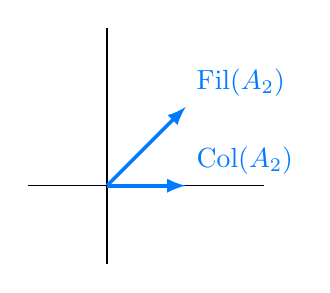
\begin{tikzpicture}[>=latex, baseline=(current bounding box.center)]
        \draw (-1,0) -- (2,0);
        \draw (0,-1) -- (0,2);
        \draw[lightblue, ->, line width=1.3] (0,0) -- (1,1) node[above right] {$\mathrm{Fil}(A_2)$};
        \draw[lightblue, ->, line width=1.3] (0,0) -- (1,0) node[above right] {$\mathrm{Col}(A_2)$};
    \end{tikzpicture}

    \item \lb{Sea $A$ una matriz $10\times 10$ que cumple $A^2=0$. Prueba que $\mathrm{Col}(A)\subseteq \mathrm{Nuc}(A)$ y en consecuencia, el rango de $A$ es menor o igual que 5.}

        Sea $v\in \mathrm{Col}(A)\longrightarrow \exists x\in \R^{10}:Ax=v$ 

        Por tanto: \[
            \underbrace{A(Ax)}_{A^2x=0}=Av,
        \] 
        es decir, $v$ es solución de  $Av=0\longrightarrow v \in \mathrm{Nuc}(A)$.

        Por el \textbf{teorema de la dimensión}, tenemos: \[
        \mathrm{dimCol}(A)+\mathrm{dimNuc}(A)=10.
        \]  
        Llamemos: \[
        \mathrm{dimCol}(A)=r\quad(\text{el rango de $A$}).
        \] 
        Entonces: \[
            \mathrm{dimNuc}(A)=10-r.
        \] 
        Dado que $\mathrm{Col}(A)\subseteq\mathrm{Nuc}(A)$, se cumple: \[
        r\le \mathrm{dimNuc}(A).
        \] 
        Sustituyendo $\mathrm{dimNuc}(A)$, se cumple: \[
        r\le \mathrm{dimNuc}(A).
        \] 
        Sustituyendo $\mathrm{dimNuc}(A)=10-r$, obtenemos: \[
        r\le 10-r\longrightarrow 2r\le 10\longrightarrow r\le 5.
        \] 
        Por lo tanto, el rango de $A$ es como máximo 5.
    \item \lb{Sea $A$ una matriz cuadrada invertible. Calcula una base para cada uno de los subespacios fundamentales de las matrices $A$ y $B=\begin{bmatrix} 
                A & A
    \end{bmatrix} $.} 

    \textbf{Subespacios fundamentales de $A$}

    Dado que $A$ es invertible:
    \begin{enumerate}[label=\arabic*)]
        \item $\mathrm{Col}(A)$:
            \begin{itemize}[label=\textbullet]
                \item Como $A$ es invertible, sus columnas forman una base de $\R^n$.
                \item Base: Las columnas de $A$.
            \end{itemize}
        \item $\mathrm{Fil}(A)$:
            \begin{itemize}[label=\textbullet]
                \item Dado que $A$ es invertible, sus filas abarcan también todo  $\R^n$.
                \item Base: Las filas de $A$.
            \end{itemize}
        \item $\mathrm{nuc}(A)$ ;
            \begin{itemize}[label=\textbullet]
                \item Dado que $A$ es invertible,  $Ax=0$ solo tiene la solución trivial  $x=0$.
                \item Base:  $\varnothing$ (dimensión 0).
            \end{itemize}
        \item $\mathrm{nuc}(A^\intercal)$:
            \begin{itemize}[label=\textbullet]
                \item Dado que $A$ es invertible,  $A^\intercal y=0$ también tiene solo la solución trivial $y=0$ 
                \item Base:  $\varnothing$ (dimensión 0).
            \end{itemize}
    \end{enumerate}
    \textbf{Subespacios fundamentales de $B=\begin{bmatrix} 
            A & A 
    \end{bmatrix} $} 

    La matriz $B$ tiene tamaño $n\times 2n$. Analices sus subespacios fundamentales:
    \begin{enumerate}[label=\arabic*)]
        \item $\mathrm{Col}(B)$:
            \begin{itemize}[label=\textbullet]
                \item Las columans de $B$ son combinaciones lineales de las columnas de $A$. Como $A$ es invertible, sus columnas ya abarcan todo  $\R^n$.
                \item Base: Las columnas de $A$.
            \end{itemize}
        \item $\mathrm{Fil}(B)$:
            \begin{itemize}[label=\textbullet]
                \item Las filas de $B$ son las mismas que las filas de $A$ duplicadas, pero no generan un espacio mayor que el de $A$.
                \item Base: Las filas de  $A$.
            \end{itemize}
        \item $\mathrm{Nuc}(B)$:
            \begin{itemize}[label=\textbullet]
                \item Resolviendo $Bx=0$, donde  $B=\begin{bmatrix} 
                        A & A 
                \end{bmatrix} $ :
                \[
                \begin{bmatrix} 
                    A & A 
                \end{bmatrix} \begin{bmatrix} 
                x_1\\ x_2 
                \end{bmatrix} =0\longrightarrow A(x_1+x_2)=0.
                \] 
                Como $A$ es invertible,  $x_1+x_2=0$, es decir, $x_1=-x_2$. Esto implica que: \[
                \begin{bmatrix} 
                x_1\\ x_2 
                \end{bmatrix} =\begin{bmatrix} 
                -x_2\\ x_2 
                \end{bmatrix} =x_2\begin{bmatrix} 
                -1\\ 1 
                \end{bmatrix} .
                \] 
            \item Base: $\left<(-1,1) \right>$.
            \end{itemize}
        \item $\mathrm{Nuc}(B^\intercal)$ :
            \begin{itemize}[label=\textbullet]
                \item Resolviendo $B^\intercal y=0$, donde: \[
                B^\intercal=\begin{bmatrix} 
                A^\intercal\\ A^\intercal 
                \end{bmatrix} .
                \] 
                Esto implica que: \[
                \begin{bmatrix} 
                A^\intercal\\ A^\intercal 
                \end{bmatrix} y=0\longrightarrow A^\intercal y_1=0\text{ y }A^\intercal y_2=0.
                \] 
                Como $A$ es invertible,  $A^\intercal y=0$ solo tiene la solución trivial. Por lo tanto, el espacio nulo a la izquierda es trivial.
            \item Base: $\varnothing$.
            \end{itemize}
    \end{enumerate}
    \item \lb{Sin calcular la matriz $A$, encuentra bases para sus cuatro subespacios fundamentales \[
    A=\begin{bmatrix} 
        1 & 0 & 0\\
        6 & 1 & 0\\
        9 & 8 & 1
    \end{bmatrix}\begin{bmatrix} 
        1 & 2 & 3 & 4\\
        0 & 1 & 2 & 3\\
        0 & 0 & 1 & 2
    \end{bmatrix}  
    \] } 
\item \lb{Halla una base del subespacio de $\R^4$ dado por el núcleo de $A$, donde \[
A=\begin{bmatrix} 
    3 & 0 & 1 & 2\\
    1 & 1 & 0 & 1 
\end{bmatrix} 
\]Comprueba que el vector $(1,1,1-2)$ pertenece a $\mathrm{Nuc}(A)$ y calcula sus coordenadas respecto de la base obtenida.}

    \begin{enumerate}[label=Paso \arabic*:]
        \item Calcular el núcleo de $A$

            El núcelo de  $A$ es el conjunto de vectores $x \in \R^4$ tales que $Ax=0$. Resolvemos el sistema homogéneo  $Ax=0$:  \[
            Ax=\begin{bmatrix} 
                3 & 0 & 1 & 2\\
                1 & 1 & 0 & 1
            \end{bmatrix} \begin{bmatrix} 
            x_1\\ x_2\\ x_3\\ x_4 
            \end{bmatrix} =\begin{bmatrix} 
            0\\ 0 
            \end{bmatrix} \longrightarrow \begin{cases}
                3x_1+x_3+2x_4=0\\
                x_1+x_2+x_4=0
            \end{cases}
            \] 
        \item Resolver el sistema

            De la segunda ecuación: \[
            x_2=-x_1-x_4.
            \] 
            Sustituyendo $x_2$ en la primera ecuación: \[
            3x_1+x_3+2x_4=0\longrightarrow x_3=-3x_1-2x_4.
            \] 
            Ahora expresamos $x$ en función de $x_1$ y $x_4$: \[
            x=\begin{bmatrix} 
            x_1\\ x_2\\x_3\\x_4 
            \end{bmatrix} =\begin{bmatrix} 
            x_1\\ -x_1-x_4\\-3x_1-2x_4\\x_4 
            \end{bmatrix}=x_1\begin{bmatrix} 
            1\\-1\\3\\0 
            \end{bmatrix}+x_4\begin{bmatrix} 
            0\\-1\\-2\\1 
            \end{bmatrix}.
            \] 
        \item Base del núcleo de $A$

            Los vectores generadores del núcleo son:  \[
            v_1=\begin{bmatrix} 
            1\\-1\\-3\\0 
            \end{bmatrix},\quad v_2=\begin{bmatrix} 
            0\\-1\\-2\\1 
            \end{bmatrix}.  
            \] 
            Por lo tanto, una base del núcleo de $A$ es:  \[
            \mathcal{B}_{\mathrm{Nuc}(A)}= <(1,-1,-3,-0),(0,-1,-2,1)>.
            \] 
        \item Verficiar que $(1,1,1,-2)\in \mathrm{Nuc}(A)$ 

            Sea $x=(1,1,1,-2)$. Comprobamos si  $Ax=0$:  \[
            Ax=\begin{bmatrix} 
                3 & 0 & 1 & 2\\
                1 & 1 & 0 & 1
            \end{bmatrix} \begin{bmatrix} 
            1\\1\\1\\-2 
            \end{bmatrix}=\begin{bmatrix} 
            3+1-4\\ 1+1-2 
            \end{bmatrix}=\begin{bmatrix} 
            0\\ 0 
            \end{bmatrix}.
            \] 
            Por lo tanto, $x \in \mathrm{Nuc}(A)$.
        \item Coordenadas de $(1,1,1,-2)$ respecto de la base $\mathcal{B}_{\mathrm{Nuc}(A)}$ 

            Queremos expresar $(1,1,1,-2)$ como combinación lineal de  $v_1$ y $v_2$: \[
                (1,1,1,-2)=c_1v_1+c_2v_2,
            \] donde: \[
            c_1\begin{bmatrix} 
            1\\-1\\-3\\0 
            \end{bmatrix}+c_2\begin{bmatrix} 
            0\\-1\\-2\\1 
            \end{bmatrix}=\begin{bmatrix} 
            1\\1\\1\\-2 
            \end{bmatrix}\longrightarrow \begin{cases}
                c_1=1\\
                -c_1-c_2=1\\
                -3c_1-2c_2=1\\
                c_2=-2
            \end{cases}.   
            \] 
            De la primera y cuarta ecuación: \[
            c_1=1,\quad c_2=-2.
            \] 
            Verificamos con las demás ecuaciones: \[
            \begin{array}{l}
                -1\cdot 1-1\cdot (-2)=-1+2=1\quad\lb{\checkmark}\\
                -3\cdot 1-2\cdot (-2)=-3+4=1\quad \lb{\checkmark} 
            \end{array}
            \] 
            Por lo tanto, las coordenadas de $(1,1,1,-2)$ respecto de la base son:  \[
                (1,1,1,-2)=1\cdot v_1-2\cdot v_2.
            \] 
    \end{enumerate}
\item \lb{Dadas las siguientes bases de $\R^4$ \[
\begin{array}{c}
    \mathcal{B}_1=\{v_1=(1,1,0,0),v_2=(0,1,0,0),v_3=(0,0,1,1),v_4=(0,0,0,1)\} \\
    \mathcal{B}_2=\{w_1=(1,2,0,0),w_2=(0,1,2,-1),w_3=(0,1,1,1),w_4=(0,1,2,0)\}
\end{array}
\]encuentra la matriz de cambio de base de $\mathcal{B}_1$ y $\mathcal{B}_2$ y la del cambio inverso. ¿Qué coordenadas tiene el vector $3v_1-v_3+2v_2$ con respecto a la base $\mathcal{B}_2$? ¿Qué coordenadas tiene el vector $3w_1-w_3+2w_2$ con respecto a la base $\mathcal{B}_1$?} 

\item \lb{Calcula una base y unas ecuaciones implícitas de $U+V$, donde  \[
\begin{array}{c}
    U=\left<(1,2,3,4,5),(5,4,3,2,1),(-1,0,1,2,3) \right>\\
    V=\left\{ (x,y,z,r,s): \begin{array}{l}
        3x+r=2y\\
        3x+s=2y
    \end{array} \right\} 
\end{array}
\] } 
\end{enumerate}
\end{document}

